%% 
%% Copyright 2007-2020 Elsevier Ltd
%% 
%% This file is part of the 'Elsarticle Bundle'.
%% ---------------------------------------------
%% 
%% It may be distributed under the conditions of the LaTeX Project Public
%% License, either version 1.2 of this license or (at your option) any
%% later version.  The latest version of this license is in
%%    http://www.latex-project.org/lppl.txt
%% and version 1.2 or later is part of all distributions of LaTeX
%% version 1999/12/01 or later.
%% 
%% The list of all files belonging to the 'Elsarticle Bundle' is
%% given in the file `manifest.txt'.
%% 

%% Template article for Elsevier's document class `elsarticle'
%% with numbered style bibliographic references
%% SP 2008/03/01
%%
%% 
%%
%% $Id: elsarticle-template-num.tex 190 2020-11-23 11:12:32Z rishi $
%%
%%
\documentclass[preprint,12pt]{elsarticle}

%% Use the option review to obtain double line spacing
%% \documentclass[authoryear,preprint,review,12pt]{elsarticle}

%% Use the options 1p,twocolumn; 3p; 3p,twocolumn; 5p; or 5p,twocolumn
%% for a journal layout:
%% \documentclass[final,1p,times]{elsarticle}
%% \documentclass[final,1p,times,twocolumn]{elsarticle}
%% \documentclass[final,3p,times]{elsarticle}
%% \documentclass[final,3p,times,twocolumn]{elsarticle}
%% \documentclass[final,5p,times]{elsarticle}
%% \documentclass[final,5p,times,twocolumn]{elsarticle}

%% For including figures, graphicx.sty has been loaded in
%% elsarticle.cls. If you prefer to use the old commands
%% please give \usepackage{epsfig}

%% The amssymb package provides various useful mathematical symbols
\usepackage{amssymb}
\usepackage{longtable}
\usepackage{array}
\usepackage{mdframed}
\usepackage{listings}
\usepackage{xcolor}
\usepackage{graphicx}
\usepackage{rotating}
\usepackage{tabularx}
\usepackage{booktabs}

%% The amsthm package provides extended theorem environments
%% \usepackage{amsthm}

%% The lineno packages adds line numbers. Start line numbering with
%% \begin{linenumbers}, end it with \end{linenumbers}. Or switch it on
%% for the whole article with \linenumbers.
%% \usepackage{lineno}

\journal{Nuclear Physics B}

\begin{document}

\begin{frontmatter}

%% Title, authors and addresses

%% use the tnoteref command within \title for footnotes;
%% use the tnotetext command for theassociated footnote;
%% use the fnref command within \author or \address for footnotes;
%% use the fntext command for theassociated footnote;
%% use the corref command within \author for corresponding author footnotes;
%% use the cortext command for theassociated footnote;
%% use the ead command for the email address,
%% and the form \ead[url] for the home page:
%% \title{Title\tnoteref{label1}}
%% \tnotetext[label1]{}
%% \author{Name\corref{cor1}\fnref{label2}}
%% \ead{email address}
%% \ead[url]{home page}
%% \fntext[label2]{}
%% \cortext[cor1]{}
%% \affiliation{organization={},
%%             addressline={},
%%             city={},
%%             postcode={},
%%             state={},
%%             country={}}
%% \fntext[label3]{}

\title{Terramycelium: A Complex Adaptive Reference Architecture for Big Data Sytems}

%% use optional labels to link authors explicitly to addresses:
%% \author[label1,label2]{}
%% \affiliation[label1]{organization={},
%%             addressline={},
%%             city={},
%%             postcode={},
%%             state={},
%%             country={}}
%%
%% \affiliation[label2]{organization={},
%%             addressline={},
%%             city={},
%%             postcode={},
%%             state={},
%%             country={}}

\author[inst1]{Author One}

\affiliation[inst1]{organization={Department One},%Department and Organization
            addressline={Address One}, 
            city={City One},
            postcode={00000}, 
            state={State One},
            country={Country One}}

\author[inst2]{Author Two}
\author[inst1,inst2]{Author Three}

\affiliation[inst2]{organization={Department Two},%Department and Organization
            addressline={Address Two}, 
            city={City Two},
            postcode={22222}, 
            state={State Two},
            country={Country Two}}

\begin{abstract}
%% Text of abstract
Lorem ipsum dolor sit amet, consectetur adipiscing elit, sed do eiusmod tempor incididunt ut labore et dolore magna aliqua. Ut enim ad minim veniam, quis nostrud exercitation ullamco laboris nisi ut aliquip ex ea commodo consequat. Duis aute irure dolor in reprehenderit in voluptate velit esse cillum dolore eu fugiat nulla pariatur. Excepteur sint occaecat cupidatat non proident, sunt in culpa qui officia deserunt mollit anim id est laborum.
\end{abstract}

%%Graphical abstract
% \begin{graphicalabstract}
% \includegraphics{grabs}
% \end{graphicalabstract}

%%Research highlights
\begin{highlights}
\item Research highlight 1
\item Research highlight 2
\end{highlights}

\begin{keyword}
%% keywords here, in the form: keyword \sep keyword
keyword one \sep keyword two
%% PACS codes here, in the form: \PACS code \sep code
\PACS 0000 \sep 1111
%% MSC codes here, in the form: \MSC code \sep code
%% or \MSC[2008] code \sep code (2000 is the default)
\MSC 0000 \sep 1111
\end{keyword}

\end{frontmatter}


\section{Introduction}
\label{sec:introduction}

The advent of the internet and widespread use of digital devices have sparked a profound shift in connectivity and data creation, leading to an era marked by a rapid growth in data. This period is characterised by the extensive expansion of data, which presents difficulties for traditional data processing systems and necessitates inventive methods in data architecture \cite{AtaeiACIS,AtaeiBigDataEnvirons}. The vast amount, variety, and rapid generation of data in the current digital environment necessitate innovative solutions, particularly in the field of Big Data (BD).

Data needs have dramatically evolved, transitioning from basic business intelligence (BI) functions, like generating reports for risk management and compliance, to incorporating machine learning across various organisational facets \cite{ataei2023towards}. These range from product design with automated assistants to personalised customer service and optimised operations.  Also, as machine learning becomes more popular, application development needs to change from rule-based, deterministic models to more flexible, probabilistic models that can handle a wider range of outcomes and need to be improved all the time with access to the newest data. This evolution underscores the need to reevaluate and simplify our data management strategies to address the growing and diverse expectations placed on data.

Currently, the success rate of BD projects is low. Recent surveys have identified the fact that current approaches to big data do not seem to be effectively addressing these expectations. According to a survey conducted by \cite{DataBricksSurvey}, only 13\% of organisations are highly successful in their data strategy. Additionally, a report by NewVantage Partners reveals that only 24\% of organisations have successfully converted to being data-driven, and a measly 30\% have a well-established big data strategy. These observations, additionally corroborated by research conducted by McKinsey \& Company (analytics2016age) and Gartner (Nash), emphasise the difficulties of successfully using big data in the industry. These difficulties include the lack of a clear understanding of how to extract value from data, the challenge of integrating data from multiple sources, data architecture, and the need for skilled data analysts and scientists. 

Without a well-established big data strategy, companies may struggle to navigate these challenges and fully leverage the potential of their data. One effective artefact to overcome some of these challenges is Reference Architectures (RAs) \cite{Cloutier2010}. RAs extract the essence of the practice as a series of patterns and architectural constructs and manifest it through high-level semantics. This allows stakeholders to refrain from reinventing the wheel and instead focus on utilising existing knowledge and best practices to harness the full potential of their data. While there are various BD RAs available to help practitioners design their BD systems, these RAs are overly cetnralised, lack attention to cross-cutting concerns such as privacy, security, and metadata, and may not effectively handle the proliferation of data sources and consumers.

To this end, this study presents TerrMycelium, a distributed RA designed specifically for BD systems with a focus on domain-driven design. TerrMycelium seeks to surpass the constraints of current RAs by utilising domain-driven and distributed approaches derived from contemporary software engineering. This method aims to improve the ability of BD systems to scale, be maintained, and evolve, surpassing the constraints of traditional monolithic data architectures.

The paper is structured as follows: Section~\ref{sec:background} provides an overview of the foundational concepts and technologies pertinent to BD reference architecture, aiming to forge a conceptual framework that is required for this paper. An overview of the existing research on the topic is presented in Section~\ref{sec:related_work}. The significance of reference architectures in the context of big data is explored in Section~\ref{sec:why_reference_architectures}. Section~\ref{sec:software_and_system_requirements} details the software and system requirements necessary for implementing the proposed architecture. Section~\ref{sec:theory} delves into the theoretical foundation underpinning the challenges in contemporary big data systems. The design and development of the TerrMycelium artifact are described in Section~\ref{sec:artifact}. Section~\ref{sec:discussion} examines the evaluation findings, their implications, limitations, and relevance to existing and future research. Finally, Section~\ref{sec:conclusion} summarizes the main contributions of the study, its practical implications, and suggests directions for future research.


\section{Background} \label{sec:background} 

This section offers fundamental definitions necessary for understanding the intricacies of the research. This chapter seeks to establish the conceptual framework required for comprehending the terminology utilised in the thesis. 

\subsection{Definition of Big Data} Various academic definitions have been reviewed to define BD in this research. According to Kaisler et al. (2013), Big Data (BD) refers to data that exceeds the capacity of current technologies to store, manage, and process effectively. The authors Srivastava (2018) define big data as the use of extensive data sets for managing the gathering or reporting of data that aids multiple recipients in decision-making. The phrase "Big Data" (BD) is defined by \citet{Sagiroglu2013} as referring to extensive data sets characterised by their huge size, diverse and intricate structure, and the challenges associated with storing, analysing, and visualising them for subsequent processes or outcomes. In this research, Big Data (BD) is defined as the process of identifying patterns from large datasets to achieve progress, management, and predictive analysis in specialised fields. 

\subsection{Significance of Big Data}\label{sec:The Value of Big Data} 

The importance and worth obtained from Big Data are clear. Extensive discussions on the topic are prevalent in publications, statistics, research, and conferences \cite{Chen2012}. Prominent corporations such as Google, Facebook, Netflix, and Amazon have significantly boosted this trend by major investments in BD projects (Rada, 2017). 

The Netflix Prize recommender system is a striking example of the real benefits of BD. The system utilised a wide range of data sources such as user queries, ratings, search phrases, and demographic factors to enhance its performance (Amatriain, 2013). Netflix saw a significant rise in TV series viewership and some series even quadrupled their audience by using Big Data-powered recommendation algorithms. 

The Taiwanese government effectively integrated its national health insurance database with customs and immigration statistics as part of a Big Data plan in the healthcare sector (Wang, 2020). The real-time notifications during clinical visits, based on clinical symptoms and travel history, helped identify possible COVID-19 cases proactively. Strategic data-driven initiatives greatly enhanced Taiwan's ability to manage the outbreak. Shell utilises Big Data in the field of energy exploration to enhance the decision-making process and minimise exploration expenses (Marr, 2016). 

By analysing and contrasting data from different drilling sites worldwide, judgements are directed towards places that resemble those with verified abundant resources. Before BD's integration, identifying energy resources was difficult. Conventional exploration techniques, based on interpreting seismic vibrations passing through the earth's crust, were both inaccurate and costly and time-consuming. Rolls Royce leverages Bangladesh's potential by gathering detailed performance data from sensors installed on its aircraft products. 

Wirelessly transmitted data offers valuable insights into crucial operating stages, including take-off and maintenance. By utilising this abundance of information, Rolls Royce can more precisely identify deterioration, improve diagnostic and prognosis accuracy, and efficiently decrease false alarms. subsectionReference Architectures Reference Architectures (RAs) are crucial components in modern system development, providing guidance for building, maintaining, and evolving complex systems citeCloutier2010. 

They provide a precise representation of the fundamental elements of a system and the interactions required to achieve broad goals. This clarity encourages the development of digestible modules, each focusing on certain parts of complicated issues, and offers a sophisticated platform for stakeholders to participate, contribute, and work together. The importance of RAs in IT is highlighted by the success of widely used technologies such as OAuth (OATH) and ANSI-SPARC architecture (ANSI), which have their roots in well-organized RAs. 

RAs define the characteristics of a system and influence its development. RAs stand apart by emphasising abstract features and higher levels of abstraction, which are present in any system's architecture. They strive to encapsulate the core of practice and incorporate proven patterns into unified frameworks, covering elements, attributes, and interconnections. RAs play a crucial role in BD by managing communication, controlling complexity, handling knowledge, reducing risks, promoting architectural visions, establishing common ground, improving understanding of BD systems, and enabling additional analysis. 

\subsection{Microservices and Decentralised, Distributed Architectures} 

Microservices architecture is a modern approach in software engineering that organises applications as a set of independent services that are loosely connected \cite{bucchiarone2020microservices}. This method, derived from the wider idea of Service Oriented Architectures (SOA), concentrates on creating small, self-sufficient modules that work together to create a complete application. 

According to \citeauthor{newman2021building}, microservices improve scalability, enable continuous deployment, and promote a more agile development environment. They allow teams to design, deploy, and scale components of a system separately, enhancing system resilience and enabling quick adaptability to changing requirements. Decentralised and distributed architectures are essential in today's computer environment, featuring systems that are spread out among several nodes, typically in various geographic regions. 


The architectural style, as emphasised by Richards (2015), addresses the drawbacks of conventional monolithic architectures by providing improved scalability, fault tolerance, and flexibility. Distributed systems involve the distribution of data and processing among several nodes that collaborate to execute tasks, as explained by Coulouris (2005). Decentralisation in this context is the absence of a central controlling node, choosing a more democratic and robust network structure instead. The integration of microservices in these systems signifies an advancement in software engineering. 

The shift is towards systems that are dispersed, modular, and flexible. This architectural style is well-suited for current requirements for systems that can scale, withstand challenges, and take use of the decentralised structure of modern computing environments. Implementing microservices in decentralised, distributed architectures marks a new phase in software development, emphasising the importance of flexibility, scalability, and resilience.


\section{Related Work}
\label{sec:related_work}

This section reviews significant works in BD RAs, detailing their emphasis, research methodologies, and inherent limitations, to endorse the distinctive approach of this study's domain-driven distributed RA, \textit{Terramycelium}. The Lambda design by Kiran (2015) and the Kappa architecture by Kreps (2014) are important industrial advancements in real-time analytics for big data, setting foundational principles for data processing. The architectures have faced criticism for their insufficient data management techniques, particularly concerning data quality, security, and metadata (AtaeiACIS). 

This gap is evident in domain-specific Regulatory Authorities (RAs) as those proposed by Quintero (2019) for healthcare. These RAs, while concentrating on certain domain requirements, sometimes overlook broader concerns such as privacy and interoperability. Academic research, like Viana (2014) and Paakkonen (2015), has concentrated on enhancing the conceptual comprehension of Big Data systems through proposed Reference Architectures to provide broader views on data analytics ecosystems. Yet, these recommendations frequently overlook the dynamic and pervasive features of modern data environments, particularly concerning scalability and adaptability. Ataei et al. (2022) highlighted the limitations of current BD RAs, emphasising a common trend: a substantial reliance on monolithic data pipeline architectures. 

Existing RAs' reliance is apparent due to their inefficiency in managing data quality, security, privacy, and metadata. Additionally, the inflexible framework of these systems often results in difficulties with scalability and adaptation, making it challenging for them to accommodate changes in data and technology settings. Within this framework, \textit{Terramycelium} is presented as a novel regulating agent for biological defence mechanisms. \textit{Terramycelium} addresses the major limitations of current RAs by implementing a domain-driven, distributed method. \textit{Terramycelium} advocates for decentralised data stewardship and a modular architecture, as opposed to traditional systems that usually have data management in rigid, monolithic structures. 

This approach enhances scalability and adaptability by including overarching issues such as security, privacy, and data quality into the system's architecture. The term "Terramycelium" is a significant departure from traditional BD RAs. By focusing on domain-driven design and distributed processing, it offers a scalable and adaptable framework that aligns well with current data management needs and contemporary software architecture concepts. Terramycelium not only addresses the limitations of present RAs but also emerges as a trailblazer in the progress of BD system design, paving the way for future research and development in this vital field.

\section{Research Methodology}

Various methods exist for the structured creation of RAs. \citeauthor{Cloutier2010} present a sophisticated strategy for creating RAs by gathering current architectural trends and innovations. citeauthorbayer1999pulse present a technique named PuLSE DSSA for generating RAs in product line development. The concept of a pattern-based Runtime Adaptation for service-based systems is introduced by Stricker et al. (2010), who emphasise the usage of patterns as primary entities. The authors Nakagawa et al. present a four-step method for creating and advancing RAs. 

Guided by ISO/IEC 26550 \citeauthor{wg2015iso} and \citeauthor{Derras} provide a four-phase method for creating practical risk assessment in the domain engineering and software product line environment. The authors of GALSTER2011Empirically suggest a 6-step process based on two main concepts: empirical foundation and empirical validity. Considering all these factors, an empirically-based research technique is the most suitable approach for this study. This process for RA development is preferred over others and aligns with the objectives of this study.

However, additional approaches must be incorporated into the methodology to achieve the appropriate level of rigour and relevance. Specific instructions for gathering empirical data in step 3 are absent. We were unsure how to proceed with data collection, synthesis, and modelling. \citeauthor{Nakagawa} presented research guidelines and introduced the RAModel concept. A more systematic and robust evaluation technique is needed as the methodology lacks details on how to assess the RA. To solve this issue, a case-mechanism experiment and expert opinion were used to assess the artefact.


\subsection{Step 1: Determination of RA Type}

The first step in creating the RA was choosing its kind using Angelov et al.'s classification framework, which divides RAs into standardisation RAs and facilitation RAs. This decision is fundamental as it directs the following stages of information gathering and risk assessment development. 

The classification framework, which considers context, aims, and design dimensions, was crucial in determining the most suitable RA type for the study's objectives. The method takes a systematic approach by employing key interrogatives such as 'When', 'Where', 'Who' for context, 'Why' for goals, and 'How' and 'What' for design to efficiently categorise RAs.

The study improved Angelov's classification by incorporating insights from a recent Systematic Literature Review (SLR) on Big Data Recommender Systems (BD RAs) cited as AtaeiACIS. The updated classification includes current instances, which can be found in Appendix A under the heading RA-classification. The selected Research Assistant for this project specialises in domain-driven distributed Big Data Research Analysis. The goal is to facilitate Big Data system development and enhance an efficient, adaptable data architecture. The standardisation RA is intended to be adaptable in many organisational settings.


\subsection{Step 2: Design Strategy Selection}

The design approach for the RA was influenced by the frameworks proposed by Angelov et al. (2008) and Galster et al. (2011), which describe two main methodologies: practice-driven (creating RAs from the beginning) and research-driven (building RAs based on pre-existing ones). Practice-driven RAs are uncommon and usually found in emerging areas, while research-driven RAs, which combine current designs, models, and best practices, are more common in established sectors.

This study chooses a research-driven strategy based on these ideas. The RA was created by utilising existing RAs, concrete structures, and documented best practices. This method allows for the development of a detailed design theory that combines and expands on the existing knowledge in the topic.

\subsection{Step 3: Empirical Data Collection} \label{theSLR}

Due to limitations in the study technique, we have enhanced this phase by increasing the systematicity and transparency of data gathering and synthesis using academic approaches like SLR. For this purpose we have adopted the findings from a SLR on current state of BD RAs presented by \citeauthor{ataei2022state}.

\subsection{Step4: Construction of the RA}
The construction phase of the RA was guided by the findings and elements identified in the earlier stages of the research. Based on the ISO/IEC/IEEE 42010 standard, the construction process involved selectively integrating its components.

This phase prominently featured the implementation of the Archimate modelling language, which is part of the ISO/IEC/IEEE 42010 standard. Archimate's service-oriented strategy efficiently connected the application, business, and technological layers of the RA. The incorporation of themes, theories, and patterns from the empirical data gathering phase, as detailed in sections \ref{identification-data-sources} and \ref{data-synthesis}, guaranteed that the research analysis addressed the specific demands stated in the study.

Using Archimate's various viewpoints offered a comprehensive perspective on the RA, encompassing technical, business, and consumer context views. This method, in accordance with the ideas presented by Cloutier et al. and Stricker et al., facilitated a thorough comprehension of the RA, guaranteeing its congruence with the study's goals and context.


\subsubsection{Step 5: Activating RA with variability}

Integrating variability into RAs is crucial to ensure its application within organizational-specific legislation and regional policies. Variability management is essential in Business Process Management (BPM) and Software Product Line Engineering (SPLE) to customise business processes and software artefacts according to specific contextual requirements.

Accurate identification and clear communication of variability are essential to encourage stakeholder discussion, maintain decision traceability, and aid the decision-making process \cite{czarnecki2012cool}. Data collected in previous analytical steps informs variability decision points. \citeauthor{galster2011empirically} outline three approaches to include variability into RAs: annotating the RA, constructing variability views, and forming variability models.

Current literature lacks in-depth information on the criteria for choosing a method to facilitate variability. This study utilises Archimate annotations to incorporate variability into the RA, following the method proposed by Rurua (2019). The technique involves two stages: first, developing a customised layer to encompass fundamental variability principles, and second, annotating the RA. The aim is not to list every possible variability point, but to highlight the main architectural variabilities associated to the system for architects to consider in order to improve the design and make it easier to implement the RA.

\subsection{Step 6: Evaluation of the RA}

Evaluating the RA is essential to ensure it achieves its developmental goals, especially in terms of efficacy and usefulness (Galster, 2011). Assessing a Research Article (RA) presents distinct difficulties because of its elevated level of abstraction, varied stakeholder groups, and emphasis on architectural features.

Common evaluation techniques for concrete architecture, like SAAM, ALMA, PASA, and ATAM, are not suitable for abstract architectural representations (RAs) because they heavily depend on stakeholder participation and scenario-based assessment. This requires a tailored method for evaluating RA.

This work utilises a revised evaluation method based on techniques tailored for RAs by Angelov et al. (2008) and the expanded SAAM methodology by Graaf et al. (2005). The approach includes developing a prototype of the RA inside for a case-mechanism experiment  and expert opinion as presented by \citeauthor{wieringa2014design}.

\section{Why Reference Architectures}
\label{sec:why_reference_architectures}

Viewing the system as a RA aids in comprehending its main elements, behaviour, structure, and development, which subsequently impact quality characteristics like maintainability, scalability, and performance (Cloutier). RAs can serve as a valuable standardisation tool and a means of communication that leads to specific architectures for BD systems. 

They also offer stakeholders a common set of elements and symbols to facilitate discussions and advance BD projects. Utilising RAs for system conceptualization and as a standardisation object is a common technique among those dealing with complex systems. Software Product Line (SPL) development uses RAs as generic artefacts that are customised and configured for a specific system domain. IBM and other top IT companies have continually supported the use of RAs as exemplary techniques for solving complex system design difficulties in software engineering. 

RAs often act as instruments in establishing uniformity in new areas within international standards. The BS ISO/IEC 18384-1 RA for service-oriented architectures showcases the effectiveness of RAs in establishing standardised frameworks in particular domains. This study utilises a 6-phase technique for creating the RA as outlined by Galster (2011). The six phases are as follows: 1) Determination of the kind of the RA 2) Develop a design strategy 3) Gather empirical data 4) Construct the Risk Assessment 5) Activate RA with variability 6) Assessment of the RA. 

The term "empirically grounded" means that the risk assessment (RA) should be based on known principles and then assessed for applicability and validity. These principles are not exclusive to the methods of Galster (2011); other researchers like Cloutier and Derras have also advocated for them.


\section{Software and System Requirements}
\label{sec:software_and_system_requirements}

According to \citeauthor{wieringa2014design}\cite{wieringa2014design}, the requirement specification phase is an essential step in developing a new IS or artefact. This phase involves identifying the requirements that the artefact must satisfy to meet the needs of stakeholders and achieve the desired outcomes.

\citeauthor{wieringa2014design}'s methodology distinguishes between functional requirements, which describe what the artefact should do, and non-functional requirements, which describe how the artefact should do it. Functional requirements are typically expressed as use cases, which describe the specific interactions between users and the system. Non-functional requirements may include performance requirements, security requirements, and usability requirements.

The requirement specification designed for this study is made up of the following phases: 

\begin{enumerate}
    \item Determining the type of the requirements 
    \item Determining the relevant requirements and 
    \item Identifying the right approach for categorisation of the requirements 
    \item Identifying the right approach for the presentation of the requirements 
\end{enumerate}

\subsection{Determining the type of the requirements:}

Defining and classifying software and system requirements is a common subject of debate. \citeauthor{sommerville2011software}\cite{sommerville2011software} classify requirements as three levels of abstraction; user requirements, system requirements, and design specifications. These abstractions are then mapped against user acceptance testing, integration testing, and unit testing. Nevertheless, in this study, a more general framework provided by \citeauthor{laplante2017requirements} is adopted. The adopted approach provides three types of requirements: functional, non-functional, and domain requirements. The objective of this step is to define the high-level requirements of BD systems, therefore the main focus is on non-functional and domain requirements. 

\subsection{Determining the relevant requirements:}

In an extensive effort, the NIST Big Data Public Working Group embarked on a large-scale study to extract requirements from a variety of application domains such as Healthcare, Life Sciences, Commercial, Energy, Government, and Defense \cite{Chang}. The result of this study is the formation of general requirements under seven categories. In addition, \citeauthor{volk2020identifying} categorize nine use cases of BD projects sourced from published literature using a hierarchical clustering algorithm. 

\citeauthor{AtaeiSecurity}\cite{AtaeiSecurity} focus on security and privacy requirements for BD systems, \citeauthor{yu2019components} present modern components of BD systems, using goal-oriented approaches, \citeauthor{eridaputra2014modeling} created a generic model for BD requirements, and  \citeauthor{al2016characteristics} investigate general requirements to support BD software development. 

By analyzing the result of the first SLRs, the studies discussed above and by evaluating the design and requirement engineering required for BD RAs, a set of high-level requirements based on BD characteristics is established. 

\subsection{Identifying the right approach for categorisation of the requirements:}

After clarifying the type of requirements and the relevant requirements, current BD RAs and their requirements have been assessed to increase understanding of the available BD requirement categorisation methods. A common theme among these studies connected the dot towards a common approach to classifying requirements. This approach is categorised through BD characteristics such as velocity, veracity, volume, variety, value, security and privacy \cite{ataei2022state, Bahrami2015,rad2017big,Chen2016a}.

\subsection{Determining the appropriate strategy for presenting the requirements:} A systematic strategy for presenting software and system requirements that includes informal model verification techniques is recognised due to its established use in both business and academics (Kassab, 2014). The method for illustrating functional requirements adheres to the principles stated in the ISO/IEC/IEEE standard 29148. The requirements representation is structured based on system modes, detailing the primary components of the system followed by the requirements. This technique is based on the requirement specification published for the NASA Wide-field InfraRed Explorer (WIRE) system and the Software Engineering Body of Knowledge (SEBoK). The requirements are outlined in Table~\ref{table:systemRequirements}.


\begin{longtable}{|m{1.4cm}|m{12cm}|}
  \caption{Terramycelium software and system requirements}
  \label{table:systemRequirements}\\
  \hline

          Volume &
  
          \textbf{Vol-1)}\label{vol-1} System needs to support asynchronous, streaming, and batch processing to collect data from centralised, distributed, and other sources
          
          \textbf{Vol-2)} System needs to provide scalable storage for massive data sets 
          \\
          \hline
          Velocity & 
          
          \textbf{Vel-1)} System needs to support slow, bursty, and high throughput data transmission between data sources
          
          \textbf{Vel-2)} System needs to stream data to data consumers in a timely manner
          
          \textbf{Vel-3)} System needs to be able to ingest multiple, continuous, time-varying data streams 
          
          \textbf{Vel-4)} System shall support fast search from streaming and processed data with high accuracy and relevancy 
          
          \textbf{Vel-5)} System should be able to process data in a real-time or near real-time manner 
          \\ 
  
          \hline
  
          Variety & 
  
          \textbf{Var-1)} System needs to support data in various formats ranging from structured to semi-structured and unstructured data 
          
          \textbf{Var-2)} System needs to support aggregation, standardization, and normalization of data from disparate sources
          
          \textbf{Var-3)} System shall support adaptations mechanisms for schema evolution
          
          \textbf{Var-4)} System can provide mechanisms to automatically include new data sources 
          \\
  
          \hline
  
          Value & 
          
          \textbf{Val-1)} System needs to able to handle compute-intensive analytical processing and machine learning techniques 
          
          \textbf{Val-2)} System needs to support two types of analytical processing: batch and streaming
          
          \textbf{Val-3)} System needs to support different output file formats for different purposes 
          
          \textbf{Val-4)} System needs to support streaming results to the consumers 
          \\
  
          \hline
  
          Security \& Privacy & 
          
          \textbf{SaP-1)} System needs to protect and retain the privacy and security of sensitive data 
          
          \textbf{SaP-2)} System needs to have access control, and multi-level, policy-driven authentication on protected data and processing nodes. 
          \\
  
          \hline
          
          Veracity &
          
          \textbf{Ver-1)} System needs to support data quality curation including classification, pre-processing, format, reduction, and  transformation 
          
          \textbf{Ver-2)} System needs to support data provenance including data life cycle management and long-term preservation.
          \\
          \hline
  
  \end{longtable}


\section{Theory}
\label{sec:theory}

An inflection point in mathematics is a critical point where the curvature of a curve changes direction, indicating a shift from one behaviour to another. This significant moment is characterised by the breaking down of the previous structure and the appearance of a new shape. Currently, there are concrete indicators and factors that suggest a significant change is imminent. The 2023 New Vantage Partners research indicates that investments in data are increasing and staying robust, despite possible economic challenges. However, the survey indicates that only 23.9\% of organisations describe themselves as data-driven. Prior to delving into these design theories, it is crucial to establish a precise communication mechanism for architectural structures. This study utilises the architecture definition defined in ISO/IEC 42010, which defines architecture as the underlying concepts or properties of a system within its context, manifested in its elements, relationships, and design and evolution principles.

\subsection{The monolith}

The techniques and methods of data engineering have experienced rapid growth, similar to the Cambrian explosion, yet the fundamental assumptions guiding data designs have not been significantly questioned.

As per Richards (2020), architectures can be classified into two main categories: monolithic, deployed as a single entity, and distributed, consisting of individually deployed sub-components. Currently, the majority of data architectures fall under the first type. 

Beginning with a monolith may be a straightforward and effective method for constructing a data-intensive system, but it becomes inadequate as the system grows. Although this notion is being questioned in the software engineering field, data engineering continues to be influenced by monolithic designs. Enabler technologies like data warehouses and data lakes support these concepts. Furthermore, numerous groups and publications embrace the concept of a "single source of truth."

\subsection{The data chasm}

Analytical data and operational data are two separate categories of data utilised in corporate operations. Operational data is utilised for daily corporate operations, whereas analytical data is employed for strategic decision-making by recognising patterns and trends in previous data.

The problems of current Big Data systems stem from the basic assumption of segregating operational and analytical data. Operational and analytical data have distinct characteristics and processing methods. Moving operational data distant from its source can harm its integrity, lead to organisational silos, and result in data quality problems. 

These two distinct data planes are often managed inside separate organisational hierarchies. Data scientists, business intelligence analysts, machine learning engineers, data stewards, and data engineers typically work under the guidance of the Chief Data and Analytics Officer (CDAO) to generate business value from data. Software developers, product owners, and quality assurance engineers typically collaborate with the Chief Technology Officer (CTO).

As a consequence, there are now two separate technology systems in place, requiring significant resources to connect them. Two distinct topologies and delicate integration designs have emerged due to this gap, facilitated by ETLs (Figure \ref{fig:dataPlanes}). Data extraction from operational databases is often accomplished through a batch ETL process. These ETL processes typically lack a clearly defined agreement with the operational database and solely consume its data. This emphasises the vulnerability of this system, as modifications made to operational databases can impact analytical applications downstream. As time passes, the complexity of ETL jobs grows, making them harder to maintain and leading to a decline in data quality. 

\begin{figure}[h]
  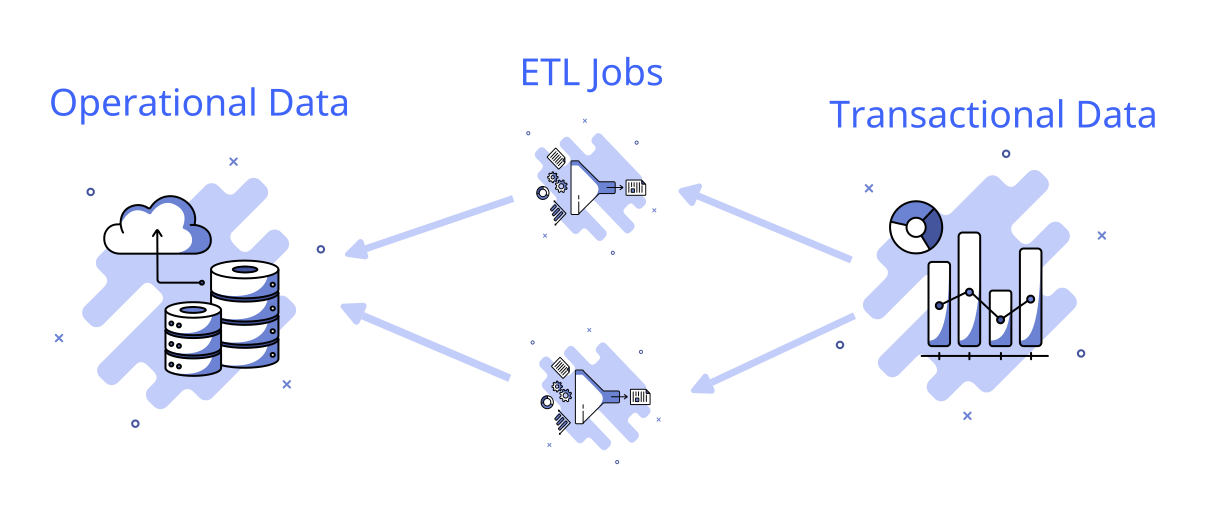
\includegraphics[width=\textwidth]{images/data-planes.png}
  \caption{The great divide of data}
  \label{fig:dataPlanes}
\end{figure}

Many technologies developed over the years are based on this notion. Although these technologies excel in managing the amount, speed, and diversity of data, current data difficulties revolve around the increase in data sources, data quality, and data architecture. 





Information is typically gathered and unified through multiple platforms. Some of this data may exceed the boundaries of the organisation. Therefore, considering the points mentioned earlier and the difficulties outlined in Section \ref{firstSLR:findings:limitationsOfCurrentRAs}, it is suggested that modern data architectures should move away from centralising data in a single large analytical database and instead focus on connecting analytical data from various sources. 

The artefact created for this study utilises earlier solutions to improve and overcome their limitations. This artefact tries to move away from highly centralised and rigid data architectures that serve as a bottleneck for coordination. This artefact aims to connect the point of data generation with its utilisation, streamlining the process. This artefact is designed to enhance agility in response to growth and successfully adapt to organisational changes. The initial architectural style of Metamycelium is as described: 


\subsubsection{Localized autonomy through domain-driven decentralisation}

Modern enterprises are facing significant complexity. A typical business consists of diverse domains with distinct structures. These domains exhibit varying rates of change and are typically segregated from one another. The business's overall synergy is determined by the relationship and evolution of various domains. 

The core of these synergies is characterised by volatility, frequent market changes, and a growing number of rules. How do modern organisations handle the effects of these developments on their data? Should they consistently update ETL tasks, develop new ETL pipelines, and merge data into operational repositories? How can firms generate reliable and high-quality data efficiently? It comes down to accepting the change in the current data environment. 

To address this complexity, one approach is to synchronise technology with business objectives. Businesses divide their challenge into smaller components within each domain, integrating technology and data into these areas. This method is well recognised in microservices architectures (Ataei, 2023). 

\subsubsection{Domain-driven design}


Central to Metamycelium is the dispersal and decentralisation of services into distinct areas with well-defined boundaries. One of the most difficult aspects of designing a distributed system is determining the architectural components on which the system should be divided. This matter has been frequently deliberated among proponents of microservices architecture, as evidenced in the citation from DataMesh. Metamycelium, influenced by domain-driven desigDataMesh places data in close proximity to the product domain it pertains to. This suggests that data is within the product domain and is a component of it \cite{laigner2021data}.

Most businesses nowadays are structured around their goods, which is the fundamental driving force behind this. These items represent the business's talents that are divided into different domains. These domains often establish their defined scope, progress at varying speeds, and are managed by interdisciplinary teams \cite{teamtopologiesSkelton}. Integrating data into these specific areas can provide a synergistic effect that enhances the handling of ongoing changes.

Communication can occur on a micro level between application developers and data engineers over user data collection in layered data structures, or on a macro level when application developers consider rebuilding their Graphql schema in a way that impacts downstream analytical services. Thus, the study integrates the concept of Domain-Driven Design (DDD) to enhance communication and improve the acceptance, precision, and significance of Metamycelium.

Domain-Driven Design (DDD) is a software development methodology that emphasises comprehending and representing the problem domain of a software application. The objective of Domain-Driven Design (DDD) is to develop software that mirrors the language, concepts, and behaviours of the problem domain, prioritising these aspects over technical factors. 

DDD can assist Metamycelium by offering a structured method for modelling and handling data that is well-matched with the application's issue domain. Domain-Driven Design (DDD) can assist data architects in obtaining a more profound comprehension of the necessary data and its structure by concentrating on the language, concepts, and behaviours of the problem domain (eridaputra 2014 modelling). DataMesh Effective communication is crucial in software development projects, as it facilitates the sharing of vital knowledge \cite{sudhakar2012model}. Data developers and business stakeholders frequently do not connect directly. Domain knowledge is conveyed through intermediaries like business analysts or project managers into a set of activities to be completed (Khrononov, 2021). This indicates the need for at least two translations from two distinct ontologies.

Each translation results in the loss of crucial subject expertise, posing a danger to the overall data quality. During a data engineering process, the requirements can become twisted, and the data engineer may lack awareness of the specific business domain or problem being addressed.

Data engineering challenges are typically complex and wide-ranging, rather than simple mathematics problems or puzzles. An organisation may choose to enhance workflows and processes by consistently making decisions based on data. However, a rigid and inflexible centralised data architecture can increase the likelihood of project failure.


\subsubsection{Complex adaptive systems}

Metamycelium architectures have characteristics similar to those of complex adaptive systems (Holland, 1992). The artefact created for this thesis is inspired by the concept that influential groups might form based on basic rules that control individual agents in a certain area. Reynolds (1987) examined a coordinated group of starling birds during the autumn season. The study revealed that each starling bird adheres to three basic rules: alignment, separation, and cohesion. The rules can be mathematically articulated as follows:

Alignment:
$$
v_i(t+1) = v_i(t) + \frac{1}{k} \sum_{j=1}^{N} (v_j(t) - v_i(t))
$$

where $v_i(t)$ is the velocity vector of bird $i$ at time $t$, $k$ is a normalization factor, and $N$ is the number of neighbouring birds.

Cohesion:
$$
v_i(t+1) = v_i(t) + \frac{1}{k} (c_i(t) - p_i(t))
$$

where $c_i(t)$ is the center of mass of the neighbouring birds, $p_i(t)$ is the position of bird $i$ at time $t$, and $k$ is a normalization factor.

Separation:
$$
v_i(t+1) = v_i(t) + \sum_{j=1}^{N} \frac{(p_i(t) - p_j(t))}{d_{ij}^2}
$$

where $p_i(t)$ is the position of bird $i$ at time $t$, $p_j(t)$ is the position of bird $j$ at time $t$, and $d_{ij}$ is the distance between birds $i$ and $j$.

Starling birds do not require a centralised orchestrator to form this intricate adaptive system. Metamycelium aims to encourage a domain-driven allocation of data ownership. This architecture is designed to offer not just operational data but also analytical data through a standard interface. The practice management software for veterinarians includes operational APIs for updating animal attributes and analytical interfaces for retrieving animal data within a specific time frame. Each domain possesses its own data.

The domain can retrieve data from other domains using a discovery mechanism, process the data, and augment its own data. Aggregate domains are created to collect data from different domains and make it available for a certain purpose. 

This aims to eliminate vertical dependency and enable teams to have local autonomy while being equipped with the appropriate amount of discovery and APIs. This architecture emphasises the concept of coequal nodes working together to accomplish the system's overarching objective, rather than relying on a centralised database managed by individuals lacking domain expertise. This idea is influenced by Domain-Driven Design (DDD) as described by Evans (2004), data mesh by Dehghani (2020), and microservices architecture by Newman (2015).

\subsubsection{Event driven services}

Metamycelium's decentralised and distributed structure poses difficulties in service communication as the network expands. At first, basic point-to-point communication via REST API calls is adequate, but it becomes inefficient as the system grows. Synchronous interactions can result in a 'distribution tax,' where one service's blocked state, generally caused by costly procedures, leads to delays in dependent services \cite{montesi2016circuit}.

Distributed systems' extensive network requirements can lead to complications such as tail latency, context switching, and gridlocks. This strong interconnection contradicts the distributed system's objectives of independence and robustness.

Metamycelium uses asynchronous event-driven communication to address these concerns. This approach allows services to publish and respond to events, so separating their interactions. Within the "publish and forget" paradigm, services broadcast events to designated topics and proceed without waiting for immediate reactions. Restaurant personnel respond to environmental signals rather than direct directives to enhance operational efficiency.

Event-driven architectures usually provide eventual consistency, which may not be ideal for some real-time stream processing situations that need immediate consistency. However, it is generally safe to assume that most data engineering tasks can effectively function within an event-driven framework.

As per Richards (2020), event-driven architectures consist of two primary topologies: 1) broker topology and 2) mediator topology. The concept of streaming platforms is further explained in the writings of Stopford (2018). Metamycelium, as a BD architecture designed for processing analytical data, eliminates several issues associated with accomplishing ACID transactions. Metamycelium utilises the architectural principles of distributed asynchronous event-driven systems with a mixed topology. Metamycelium is incorporating aspects from the broker topology, mediator topology, and several notions from streaming platforms. Metamycelium's CAP theorem prioritises partition tolerance and availability as key assurances. 

The hybrid topology consists of five main architectural components: the event, the event consumer, the event producer, the event backbone, and the eventing interface. Events are triggered by the event producer and sent to the relevant topic. The event is processed by the event broker and stored in a queue-like indexed data structure for later retrieval. Interested event consumers will listen to the topic of interest using the eventing interface. The event backbone is an internally distributed system composed of numerous event brokers. 

Event brokers are services created and provided to enable event communication via Metamycelia. The brokers are synchronised with a decentralised service coordinator. Brokers also enable the replication of subjects. Additionally, the event backbone includes a specialised event archive to ensure fault tolerance and recoverability. The purpose of this archive is to retain all events processed by the brokers for potential restoration in case of a failure. 




The components collaborate to establish a distributed, fault-tolerant, and scalable data system capable of managing both batch and stream processing, as seen in Figure \ref{fig:eventDrivenArchitecture}. 

\begin{figure}[h]
  \centering
  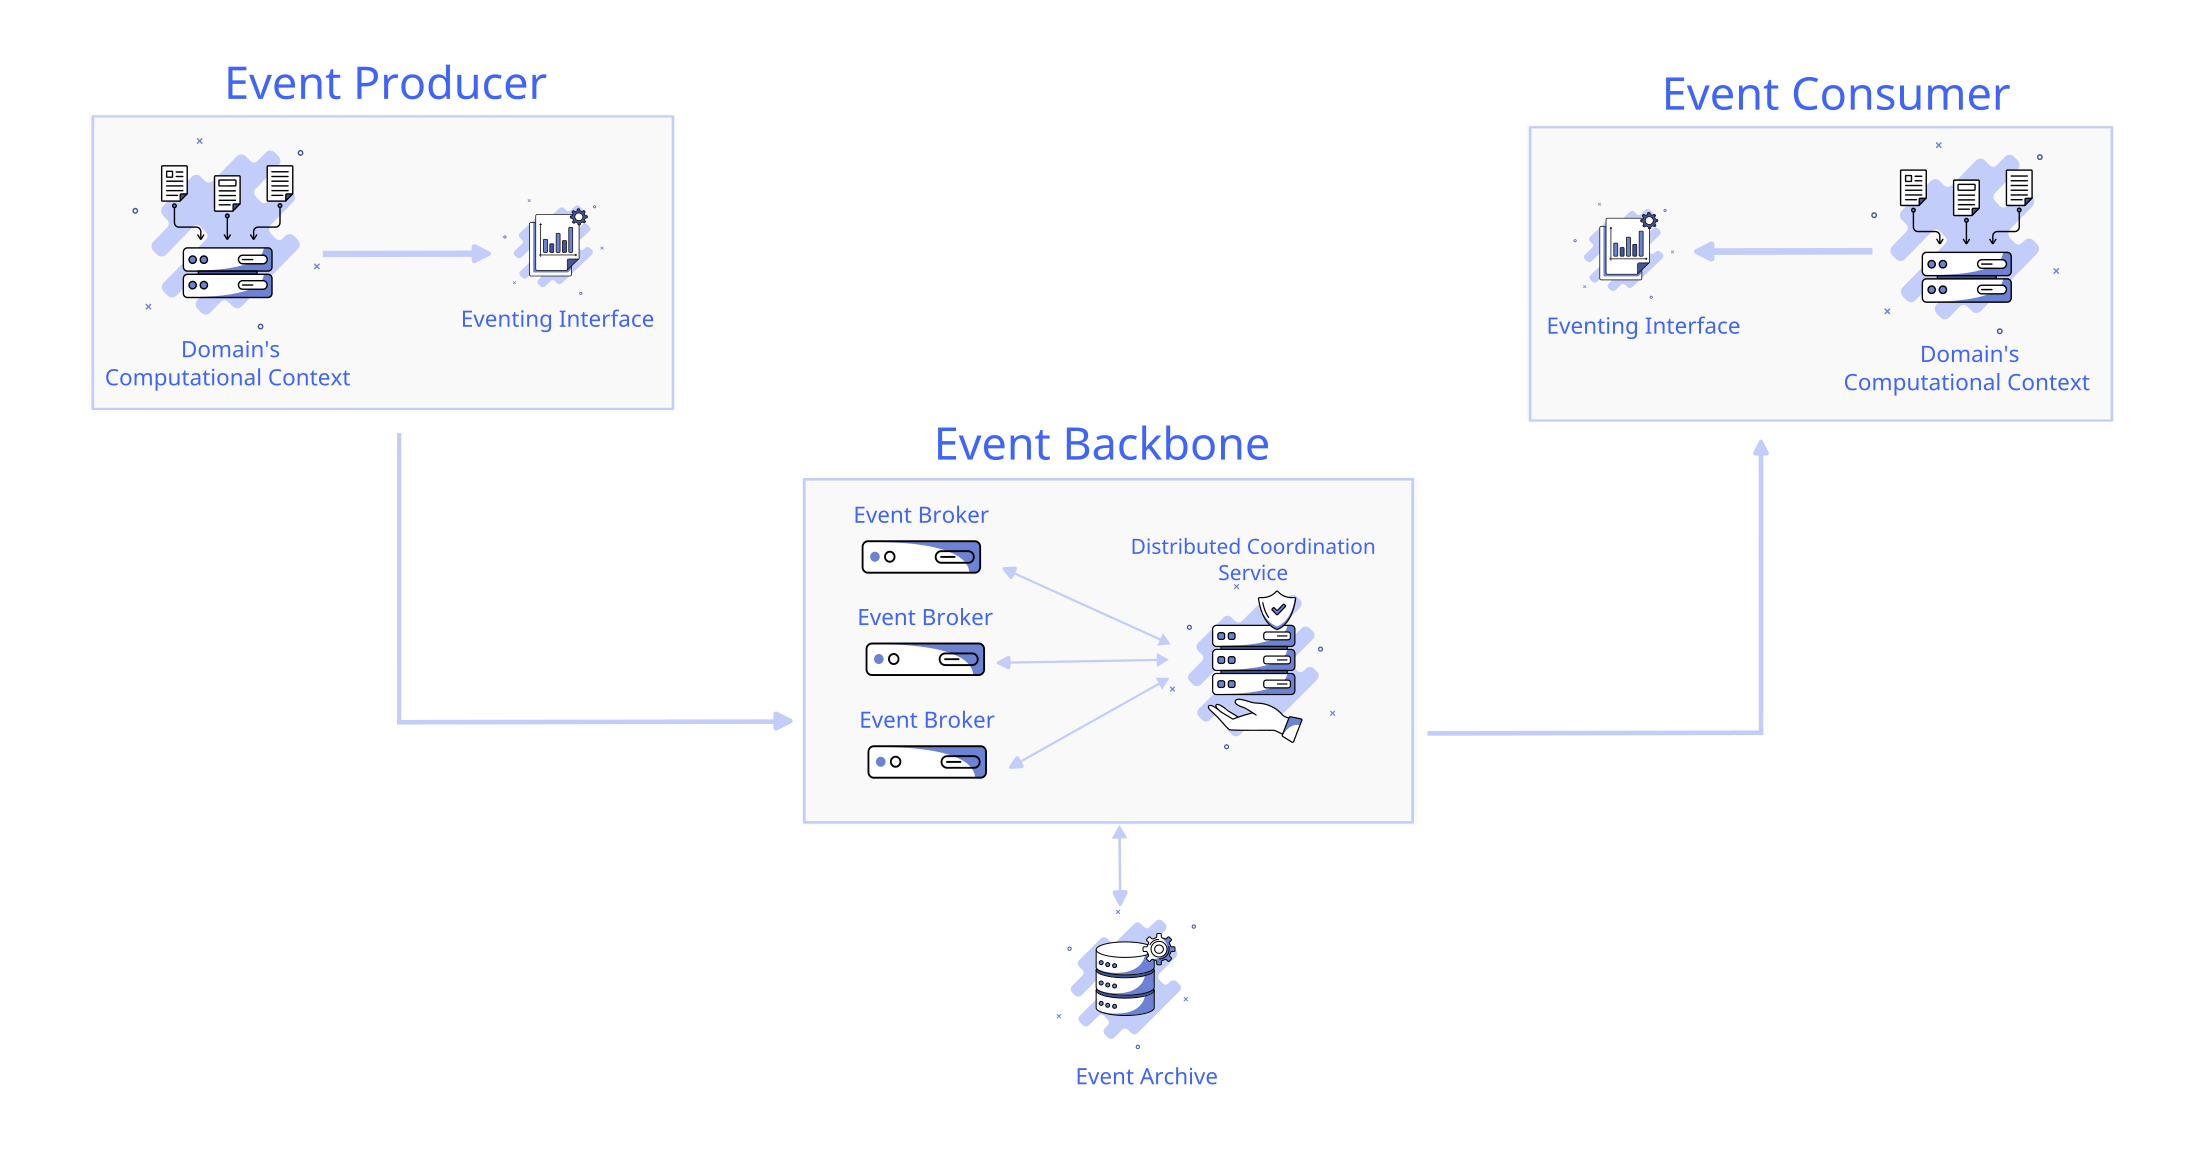
\includegraphics[width=\textwidth]{images/Event-architecture.png}
  \caption{Metamycelium Event-driven Architecture}
  \label{fig:eventDrivenArchitecture}
\end{figure}


\subsection{Architectural characteristics}

The Metamycelium architecture is distinguished by its emphasis on maintainability, scalability, fault tolerance, elasticity, and deployability. It is in line with contemporary engineering methodologies like automated deployment and continuous integration. The architecture focuses on utilising microservices, which are autonomous components that can be deployed and maintained separately.

This architecture excels in maintainability. Event-driven microservices architecture enables modular development and independent scaling, facilitating the maintenance and updating of individual components without impacting the entire system. The design also enables automated deployment processes, which help streamline upgrades and minimise manual interaction.

Scalability and elasticity are significant aspects as well. The architecture allows for horizontal scalability, enabling the addition or removal of services according to demand. This adaptability guarantees that the system can efficiently manage different workloads.

The architecture also demonstrates strong fault tolerance. Interservice communication can affect fault tolerance, however a redundant and scalable design of Metamycelium, combined with service discovery techniques, helps alleviate this problem. Microservices' standalone and single-purpose design typically results in a high level of fault tolerance.

Metamycelia's minimal deployment components and decoupled design highlight deployability. The design facilitates evolutionary transformation to correspond with contemporary business practices that demand agility and adaptability. Modular and autonomous units provide quicker updates and iterations, ensuring alignment with the ever-changing business needs.

The architecture might be rated lower in terms of cost and simplicity. The decentralised structure of Metamycelium and the possibility of higher communication overhead can create challenges in cost management and optimisation. Implementing strategies like intelligent data caching and replication can help overcome performance issues related to network calls, but managing costs is still a continuous concern.

The Metamycelium design emphasises the advantages of microservices, focusing on maintainability, scalability, fault tolerance, elasticity, and deployability. The text recognises the difficulties that come with distributed architectures and provides methods to reduce their impact. Architects need to comprehend the principles of architecture in order to skillfully traverse and capitalise on its advantages. An overview of architectural characteristics is portrayed in Table~\ref{tab:architecture-characteristics}

\begin{table}[t]
  \centering
  \caption{Metamycelium Architecture Characteristics}
  \label{tab:architecture-characteristics}
  \begin{tabular}{|l|c|}
    \hline
    \textbf{Characteristic} & \textbf{Score} \\
    \hline
    Maintainability & $\bigstar\bigstar\bigstar$ \\
    \hline
    Scalability & $\bigstar\bigstar\bigstar\bigstar$ \\
    \hline
    Fault Tolerance & $\bigstar\bigstar\bigstar$ \\
    \hline
    Elasticity & $\bigstar\bigstar\bigstar\bigstar$ \\
    \hline
    Deployability & $\bigstar\bigstar\bigstar\bigstar$ \\
    \hline
    Cost & $\bigstar\bigstar$ \\
    \hline
    Simplicity & $\bigstar$ \\
    \hline
    Performance & $\bigstar\bigstar\bigstar$ \\
    \hline
    Support for Modern Engineering Practices & $\bigstar\bigstar\bigstar\bigstar$ \\
    \hline
  \end{tabular}
\end{table}







\section{Artifact}
\label{sec:artifact}

After exploring several kernel and design theories, a solid theoretical foundation is established for creating and developing the artefact. Metamycelium is generated using Archimate and mostly showcases the RA within the technological layer. The architect has the responsibility to determine the flow and application that should be present in each node when showcasing these services in the technology layer. To ensure thoroughness, a basic business process is assumed as every software is created to fulfil a business requirement. Metamycelium should possess the flexibility needed to accommodate alternative business models, notwithstanding potential variations in the business layer across different settings.

The BD RA does not depict the architecture of any particular BD system. It functions as a versatile tool for describing, discussing, and constructing system-specific designs based on standardised principles. Metamycelium enables in-depth and insightful talks about the needs, frameworks, and functions of BD systems. The system stays vendor-neutral, providing flexibility in choosing products or services, and avoids imposing strict solutions that restrict innovation. 

To ensure thoroughness, we have assumed a basic BD business process, as all software is created to fulfil a specific business requirement. Metamycelium consists of 15 primary components and 5 variable components, as seen in Figure \ref{fig:Metamycelium}. The lowercase "a" in the top left corner of the diagram represents the auxiliary view, while the letter "m" represents the master view. When the same entity is utilised in various models, the auxiliary view is employed. This indicates that the entity already exists and is being reused. 


\begin{sidewaysfigure}
  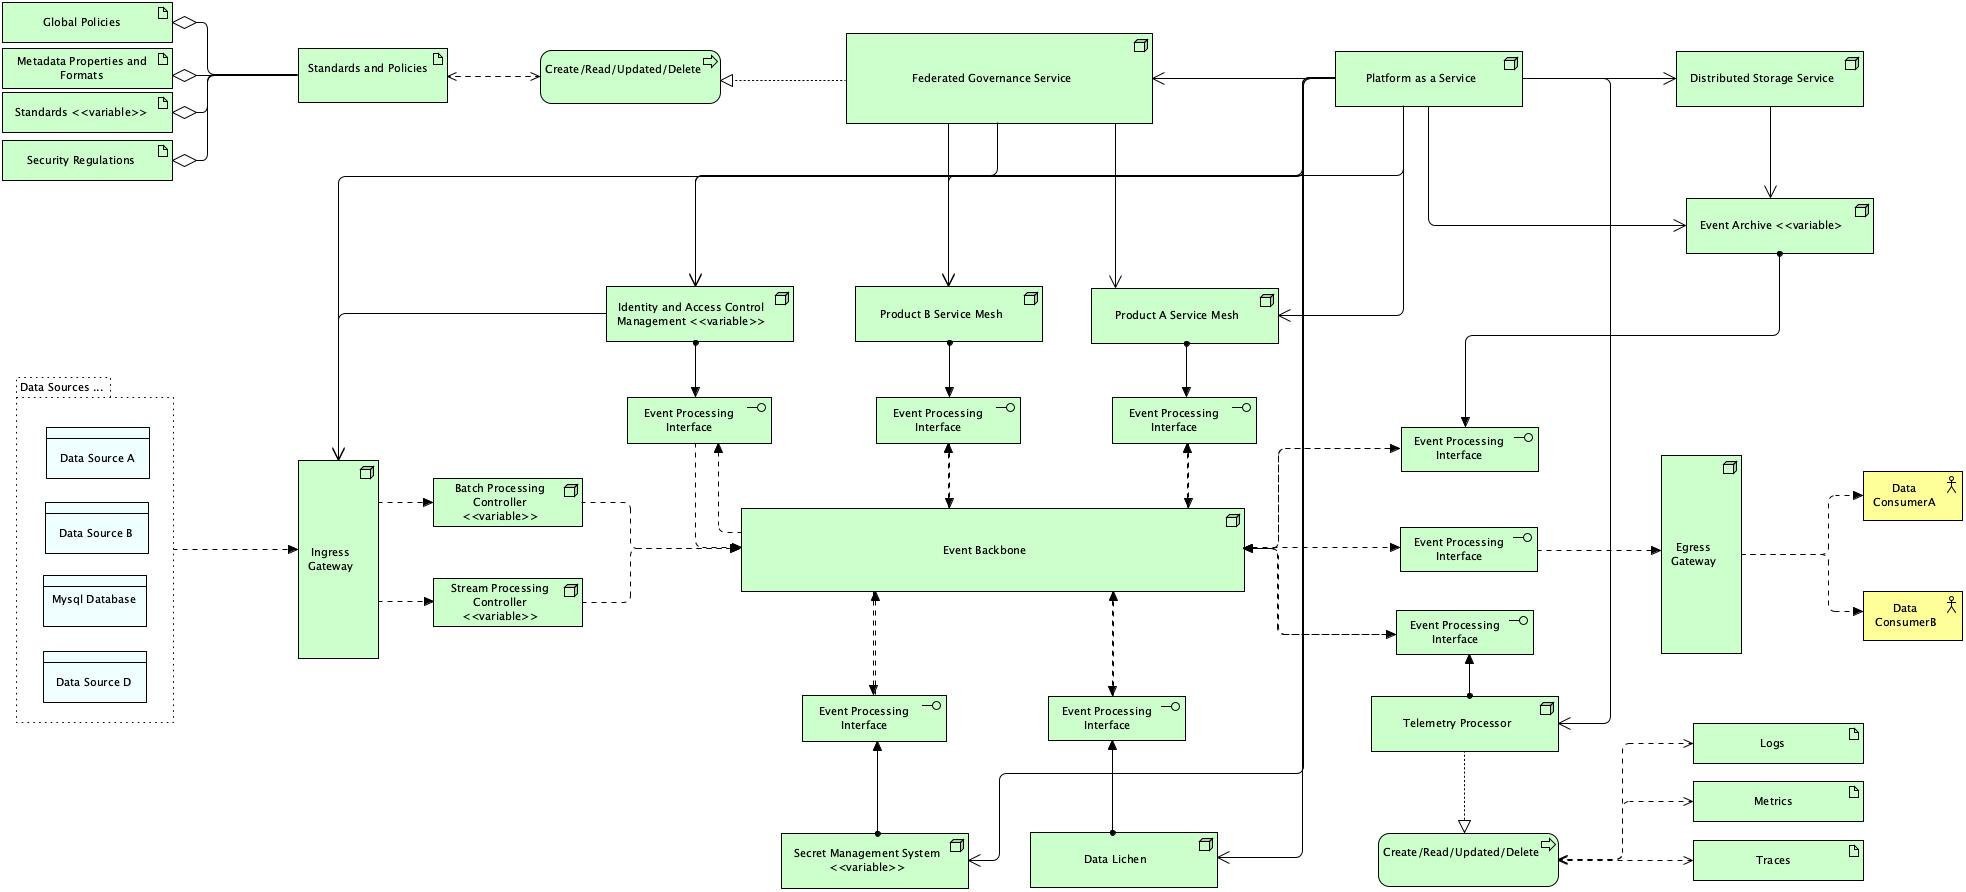
\includegraphics[width=23cm]{images/Metamycelium.jpg}
  \caption{Metamycelium}
  \label{fig:Metamycelium}
\end{sidewaysfigure}

While this business layer could vary in different contexts, Metamycelium should be able to have the elasticity required to account for various business models. To ease understanding of the RA, we sub-diagrammed the product domain in Figure \ref{fig:MetamyceliumServiceMesh}.

\begin{sidewaysfigure}
  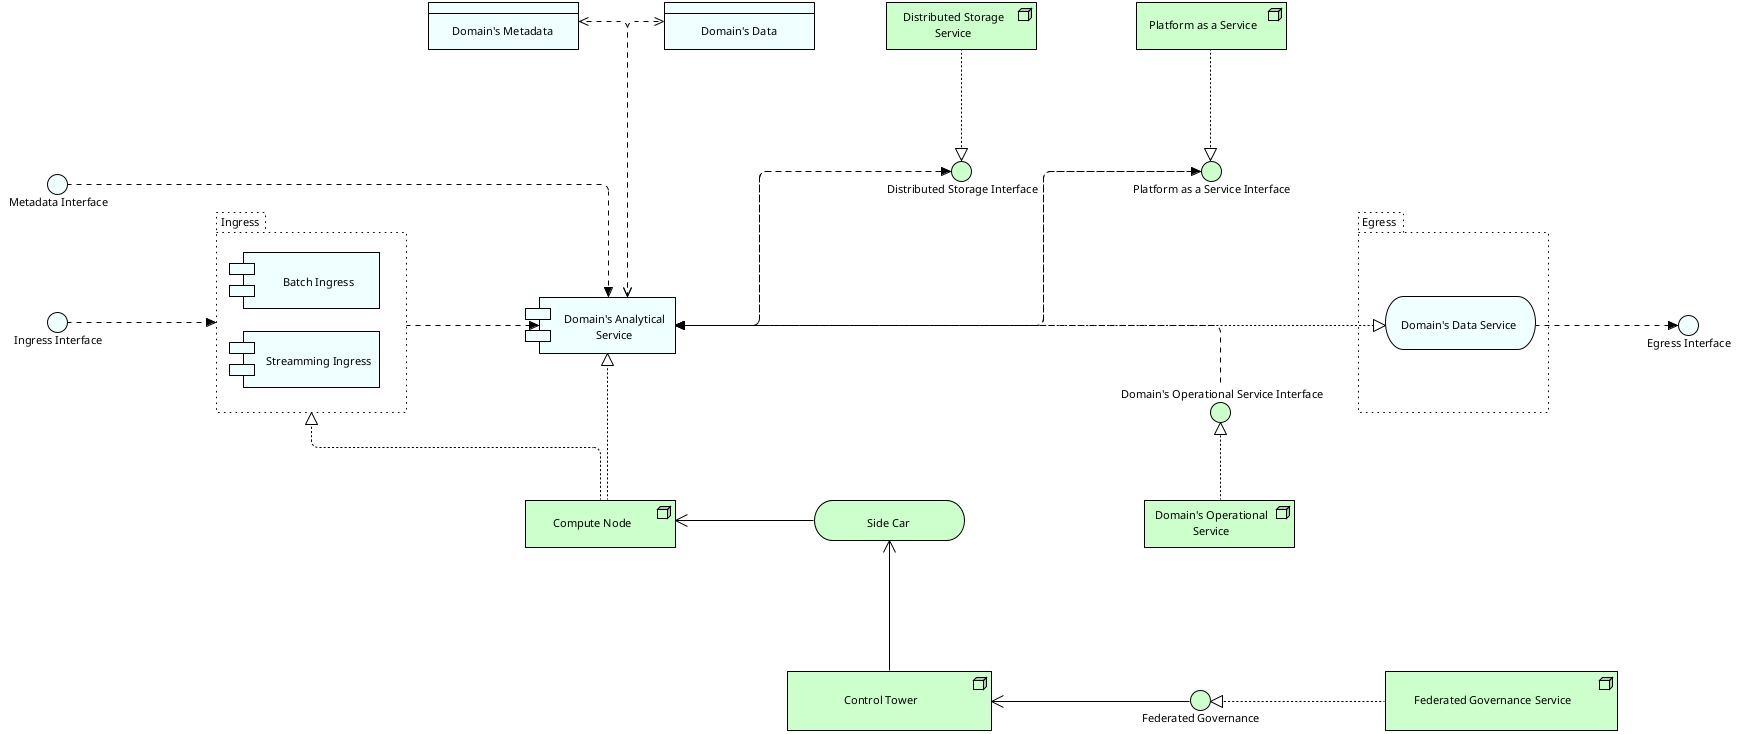
\includegraphics[width=23cm]{images/metamyceliumServiceMesh.jpg}
  \caption{Service Mesh}
  \label{fig:MetamyceliumServiceMesh}
\end{sidewaysfigure}

These components are;

\begin{enumerate}
    \item \textbf{Ingress Gateway:} The ingress gateway is pivotal in Metamycelium, acting as the main entry point for external requests. It exposes necessary ports and endpoints, intelligently load-balancing traffic to the appropriate processing controllers, thereby enhancing the system's scalability and performance.

    Security is significantly bolstered by the ingress gateway, preventing direct service access by centralizing entry and enabling the enforcement of security policies such as SSL termination and authentication. This approach secures communication with external entities and streamlines SSL processing, offloading this task from downstream services.
    
    The gateway also allows for incoming data modification or enrichment, offering customization and system integration capabilities. This architectural component simplifies monitoring and observability, concentrating metrics, logging, and tracing at a singular point for efficient analysis and compliance oversight. Additionally, it supports network segmentation, establishing a clear demarcation between public interfaces and private network resources, thus reinforcing security and control over data flow.
    

    \textit{Addresses requirements: Vol-1, Vol-2, Var-1, Var-3, Var-4, Val-1, Val-3, Val-4, SaP-1, and SaP-2.}



    \item \textbf{Batch Processing Controller:} The primary function of the batch processing controller is to manage batch events by sending them to the event backbone. The dedicated service, which may be a tiny service or a Lambda function, processes batch-processing requests and converts them into events for the event broker. Its unique characteristics enable it to handle batch requests in large quantities and asynchronously, distinguishing it from stream processing controllers.

    The batch-processing controller offers various architectural advantages. Firstly, it greatly improves monitoring capabilities, offering clearer insight into the status and performance of batch activities. This efficient monitoring simplifies problem-solving and performance evaluation, guaranteeing that batch processing adheres to defined criteria and performance standards.
    
    The batch processing controller allows for customisation and flexibility in generating batch events. It can carry out supplementary functions apart from computationally demanding activities, including data cleansing or incorporating personalised headers. Businesses can customise batch event production to meet their individual needs and expectations.
    
    A specialised controller for batch processing recognises the distinct needs and attributes of batch events, offering tailored features and enhancements. This component fulfils the criteria.

    \textit{Addresses requirements: Vel-1, Val-1, and Val-2.}
    
    \item \textbf{Stream Processing Controller:}  The stream processing controller is a crucial component in architecture, handling streaming events and dispatching them to the event backbone. It is distinct from batch processing services as it focuses on non-heavy computations optimized for stream processing requirements. It can enable stream provenance, providing insights for data governance and traceability. It can also leverage one-pass algorithms for stream analytics tasks.

    A dedicated stream processing controller allows for the association of custom attributes with stream events, enabling contextual enrichment of streaming data and differentiated treatment based on the system's nature. This enables real-time decision-making or targeted actions based on event content.
    
    Simplifying monitoring and discovery within the architecture, the controller simplifies tracking and analyzing performance, latency, and throughput of streaming events. It also enables focused monitoring of stream-specific metrics, providing valuable insights into the behavior and efficiency of the streaming data pipeline.
    
    In summary, the stream processing controller is an essential component in architectures involving streaming data due to its ability to handle high throughput, apply custom attributes, optimize computations, and simplify monitoring and discovery. 
    
    \textit{Addresses requirements: Vol-1, Vel-1, Vel-2, Vel-4, Vel-5, and Val-2.}

    
    \item \textbf{Event Processing Interface:} Event brokers are designed to achieve \emph{inversion of control}. As the company evolves and requirements emerge, the number of nodes or services increases, new regions of operations may be added, and new events might need to be dispatched. As each service has to communicate with the rest through the event backbone, each service will be required to implement its event-handling module. 
    
    This can easily turn into a spaghetti of incompatible implementations by various teams, and can even cause bugs and unexpected behaviours. To overcome this challenge, an event broker is introduced to each service of the architecture. Each service connects to its local event broker and publishes and subscribes to events through that broker. One of the key success criteria of the event broker is a unified interface that sits at the right level of abstraction to account for all services of the architecture. 
    
    Event brokers, being environmentally agnostic can be deployed to any on-premise, private or public infrastructure. This frees up engineers from having to think about the event interface they have to implement and how it should behave. Event brokers can also account for more dynamism by learning which events should be routed to which consumer applications. Moreover, event brokers do also implement circuit breaking, which means if the service they have to break to is not available and does not respond for a certain amount of time, the broker establishes unavailability of the service to the rest of the services, so no further requests come through. This is essential to preventing a ripple effect over the whole system if one system fails. 
    
    \textit{Addresses requirements: Val-1, Ver-1.} 

    \item \textbf{Event Backbone:} The event backbone is the central component of the Metamycelium, enabling communication between nodes. The distribution and clustering should be implemented to handle the system's scalability. Communication is orchestrated by coordinated activities, like to a dance ensemble. Every service monitors and responds to the event backbone, performing required actions. 
    
    This guarantees an uninterrupted exchange of data between services, ensuring that all systems are in the appropriate condition. The event backbone can combine many event streams, store events in a cache, archive events, and perform other operations, as long as it does not become overly intelligent or function as an Enterprise Service Bus (ESB) in Service-Oriented Architecture (SOA) systems. An architect should see the event backbone as a collection of interconnected nodes that address different subjects of interest. The event backbone can be monitored over time to analyse access patterns and adjusted to optimise communication efficiency.

    \textit{Addresses requirements: Vel-1, Vel-2, Vel-3, Vel-4, Vel-5, Val-1, Val-2, Ver-1, Ver-2, and Ver-3.} 
    

    \item \textbf{Egress Gateway:} The inclusion of an egress gateway in Metamycelium offers numerous advantages, especially for external data consumers. In this architecture, data consumers first interact with the discovery component, known as Data Lichen, which serves as a central hub for accessing available data domains. Once connected to Data Lichen, data consumers can navigate to the relevant data domain to retrieve the desired data.

    Furthermore, all external data consumers in the system go through a centralised secret management and centralised authentication and authorisation component. This centralised approach brings several benefits to the architecture. Firstly, it ensures a consistent and secure management of secrets, such as API keys, access tokens, or credentials, which are essential for data access and security. This centralised secret management enhances the overall system's security posture by reducing the chances of vulnerabilities or misconfigurations in secret handling.

    Secondly, the centralised authentication and authorisation component streamlines the authentication and access control processes for external data consumers. By enforcing a unified authentication mechanism, it ensures that all users are properly authenticated and authorized before accessing the system's data resources. This centralised approach simplifies the management of user access rights, improves security, and provides granular control over data access permissions.

    Thirdly, the centralised components simplify the maintenance and scalability of the system. With a single point for managing secrets, authentication, and authorisation, it becomes easier to update, monitor, and audit these components. Additionally, this architectural pattern allows for easier scaling and expansion as new data domains or data sources can be seamlessly integrated into the system with consistent authentication and authorisation mechanisms.

    Overall, the inclusion of an egress gateway in Metamycelium offers a robust and efficient approach for external data consumers. It ensures standardised data access, enhances security, simplifies maintenance, and enables scalability, making it a highly favourable and beneficial architectural design. 
    
    \textit{Addresses requirements: Vel-2, Vel-4, Val-3, Val-4, SaP-1, and SaP-2.} 
    
    \item \textbf{Product Domain Service Mesh:} Integrating a service mesh as a core element of each product's domain is an effective strategy in the architectural framework. The service mesh consists of essential components that work together to facilitate effective data processing, storage, governance, and communication inside the domain. The components consist of batch and streaming data input, analytical and operational services specific to the domain, API access to distributed storage services, an infrastructure API for platform-as-a-service modules, containers hosting the analytical service, a control tower, and integration with a federated governance service's API for policy enforcement using sidecars.

    The service mesh's effectiveness is derived from its architectural design and its capability to meet essential needs. By integrating the domain's functionalities into a service mesh, the interdependence across teams is removed, enabling greater team independence. The components of the service mesh collaborate to provide benefits like data ingestion into the analytical service domain, API connectivity to distributed storage services, container hosting for the analytical service domain, a control tower, and integration with a federated governance service's API for policy enforcement using sidecars.
    
    The service mesh architecture provides the analytical service with direct access to operational data, connecting data analytics and operational systems. The analytical service can obtain real-time insights and a comprehensive overview of the system's activities, which minimises the requirement for manual data extraction and transformation procedures. Accessing operational data directly improves the efficiency and precision of analytical services, leading to more precise analysis and well-informed decision-making.
    
    The service mesh architecture enables a cohesive perspective of the system, promoting smooth cooperation between analytics and operations teams. The system supports scalability, adapts to changes in business environments, validates data, maintains quality and integrity, and meets security and privacy standards by enforcing policies, ensuring secure communication, and implementing data governance processes.

    The service mesh's effectiveness lies in its ability to address key architectural concerns. It promotes scalability, allowing the domain to handle large volumes of data and increasing computational resources as needed (Vol-1). It facilitates rapid development and deployment of analytical capabilities (Vel-3, Vel-4, Vel-5). The service mesh architecture accommodates variability in business contexts, supporting the diverse needs and requirements of different product domains (Var-1, Var-2, Var-3). It ensures data validation, quality, and integrity by leveraging advanced analytics and processing techniques (Val-1, Val-2, Val-3, Val-4). Security and privacy requirements are fulfilled through policy enforcement, secure communication, and data governance mechanisms (Sap-1, SaP-2). 
    
    Finally, the service mesh architecture allows for the verification of system behaviour, enabling efficient testing, monitoring, and verification of the domain's analytical outputs (Ver-1, Ver-2, Ver-3).

    \textit{Addresses requirements: Vol-1, Vel-3, Vel-4, Vel-5, Var-1, Var-2, Var-3, Val-1, Val-2, Val-3, Val-4, Sap-1, SaP-2} 
  
    \item  \textbf{Federated Governance Service:} Metamycelium's distributed architecture comprises multiple independent services with distinct lifecycles, developed and deployed by autonomous teams. To ensure coherence and prevent interface conflicts without centralizing control, a global federated governance is essential. This governance model standardizes services, enhancing their interoperability and facilitating team collaboration. It also mitigates risks, such as non-compliance with GDPR, by establishing a unified framework of global policies, metadata standards, API standards, and security protocols. This framework not only supports organizational practices but also aligns with external regulations, safeguarding against potential fines and security threats. The federated governance service, comprising components like global policies, metadata standards, and security regulations, plays a pivotal role in maintaining the architecture's integrity and adaptability, indirectly impacting all requirements. This component can indirectly affect all requirements.

    \textit{Addresses requirements: All.}     

    \item \textbf{Data Lichen:} With an increasing number of products, more data is accessible for users, leading to enhanced interoperability but also posing greater challenges for maintenance. Without an automated method for different teams to obtain their desired data, a tightly connected and sluggish data culture would develop. To overcome these obstacles and enhance the ability to find, work together, and navigate with guidance, the Data Lichen should be put into practice. Gartner has identified data discovery mechanisms such as Data Lichen as essential tools. These mechanisms facilitate improved communication dynamics, quicker data access through services, and intelligent collaboration among services.

    \textit{Addresses requirements: Vel-4, Var-1, Var-3, and Var-4.} 
    
    
    \item \textbf{Telemetry Processor:}  The decentralised architecture of Metamycelium poses challenges for debugging, fault identification, and maintenance as it requires tracking transactions across several services. Consolidating the handling of telemetry data in Metamycelium provides architectural advantages by streamlining data processing, offering a cohesive perspective of logs, metrics, and traces, facilitating thorough analysis and correlation, and guaranteeing optimal resource distribution. Centralising the service guarantees uniform monitoring and governance processes throughout the architecture, encouraging compliance with best practices.

    The centralised service can act as a data source for different users, like the Data Lichen, which uses processed telemetry data to create important insights. This service may process data that can be used by customised systems and dashboards, offering adaptability and scalability to fulfil particular business needs. This promotes a data-driven environment, enabling individuals to get valuable information and insights from the analysed telemetry data. The flexibility and ease of access to the telemetry data increase the benefits of the centralised service in the larger BD framework.

    \textit{Addresses requirements: Vol-1, Vel-1, Val-1, and Ver-1.} 


    \item \textbf{Event Archive:} As the quantity of services expands, the subjects in the event backbone rise, leading to a surge in the number of events. If such circumstances occur, there is a possibility of failure leading to a timeout and subsequent loss of a sequence of events. This can lead to the system being in an incorrect state, causing a harmful chain reaction that affects all services. Metamycelium often addresses these issues by utilising an event archive. The event archive is in charge of recording occurrences for future retrieval in case of failure. 
    
    During a blackout in a specific area, if the event backbone is down, it can restore itself and return the system to its correct state by retrieving events from the event archive. The event interface manages circuit breaking to prevent services from sending additional requests to the backbone while it is not functioning. The determination of the duration till expiration and the selection of events to be stored are made according to the specific circumstances in which Metamycelium is utilised.


    \textit{Addresses requirements: Vol-1, Vel-1, Val-1, and Ver-1.} 

    \item \textbf{Distributed Storage Service:} Metamycelium supports decentralised and distributed systems but does not require each product domain to have its unique data store. To avoid duplication, conflicting data storage methods, reduced interoperability across services, and absence of consistent data storage techniques. The distributed storage service is intended to store vast amounts of data in its original format until it is ready to be retrieved for analysis and other uses. 
    
    Data can be stored in the distributed storage service with the appropriate domain ownership before being accessed and used by different services. Data of various structures, such as structured, semi-structured, unstructured, and pseudo-structured, can be stored in a distributed storage service before being processed in batches or streams. However, not all data should be sent straight to this service; the data flow depends on the specific context in which the system operates.
    
    \textit{Addresses requirements: Vol-2, Vel-1, Var-1, Var-3, Var-4, Val-3.} 


    \item \textbf{Platform as a Service:} The Platform as a Service (Paas) component acts as a central hub providing an API to all other system components. This PaaS component is essential for facilitating the independence and expandability of the entire infrastructure.

    The primary design value of this PaaS component is its capacity to simplify the underlying infrastructure difficulties. By offering a standardised API, each component can autonomously handle and allocate necessary resources like computing power, storage, and networking without having to deal with the complex specifics of the underlying infrastructure. This abstraction layer encourages a minimal connection between components, making it simpler to create, deploy, and maintain the entire system.
    
    The PaaS component places importance on scalability and elasticity as key design values. It allows for the flexible allocation and deallocation of resources according to the changing requirements of diverse data domains. The PaaS component facilitates effective infrastructure utilisation by providing an API that allows components to request resources as required. The system may adjust resources as needed to maintain peak performance and cost efficiency throughout the whole architecture.
    
    Data domains can utilise the PaaS API to request, set up, and oversee resources, allowing them to function autonomously and effectively. Decentralising infrastructure management improves agility and flexibility in the system.
    
    \textit{Addresses requirements: SaP-1, SaP-2, Var-1, Var-3, Var-4, Vel-1, and Vol-2.} 

    \item \textbf{Identity and Access Management:} The role of the Identity and Access Management (IAM) component is to guarantee secure and regulated access to the system's resources and data. The concept includes a range of architectural principles necessary for upholding data integrity, privacy, and regulatory compliance.

    The IAM component places significant emphasis on authentication and authorization as core design concepts. The system offers strong methods to verify the identities of users, components, and services in the structure, guaranteeing that only approved entities can get the resources and carry out particular tasks. These measures aid in preventing unauthorised access, reducing security risks, and protecting sensitive data.
    
    Another architectural value of the IAM component is its emphasis on centralised user and access management. It acts as a centralised authority for overseeing user identities, responsibilities, and permissions throughout Metamycelium. Centralization optimises access control management, speeds user onboarding and offboarding, and maintains uniform security policy enforcement system-wide.
    
    The IAM component guarantees meticulous access control and privilege management, enabling the creation of precise access policies. The system enables strong authentication using standard protocols such as OAuth and SAML, simplifying user access through Single Sign-On (SSO). It supports audits by recording access occurrences, strengthening compliance, security oversight, and incident management. The Figure~\ref{diagram:IAM} provides a detailed representation of how the component functions and how it interacts with other aspects of the system.

    \begin{figure}[h]
        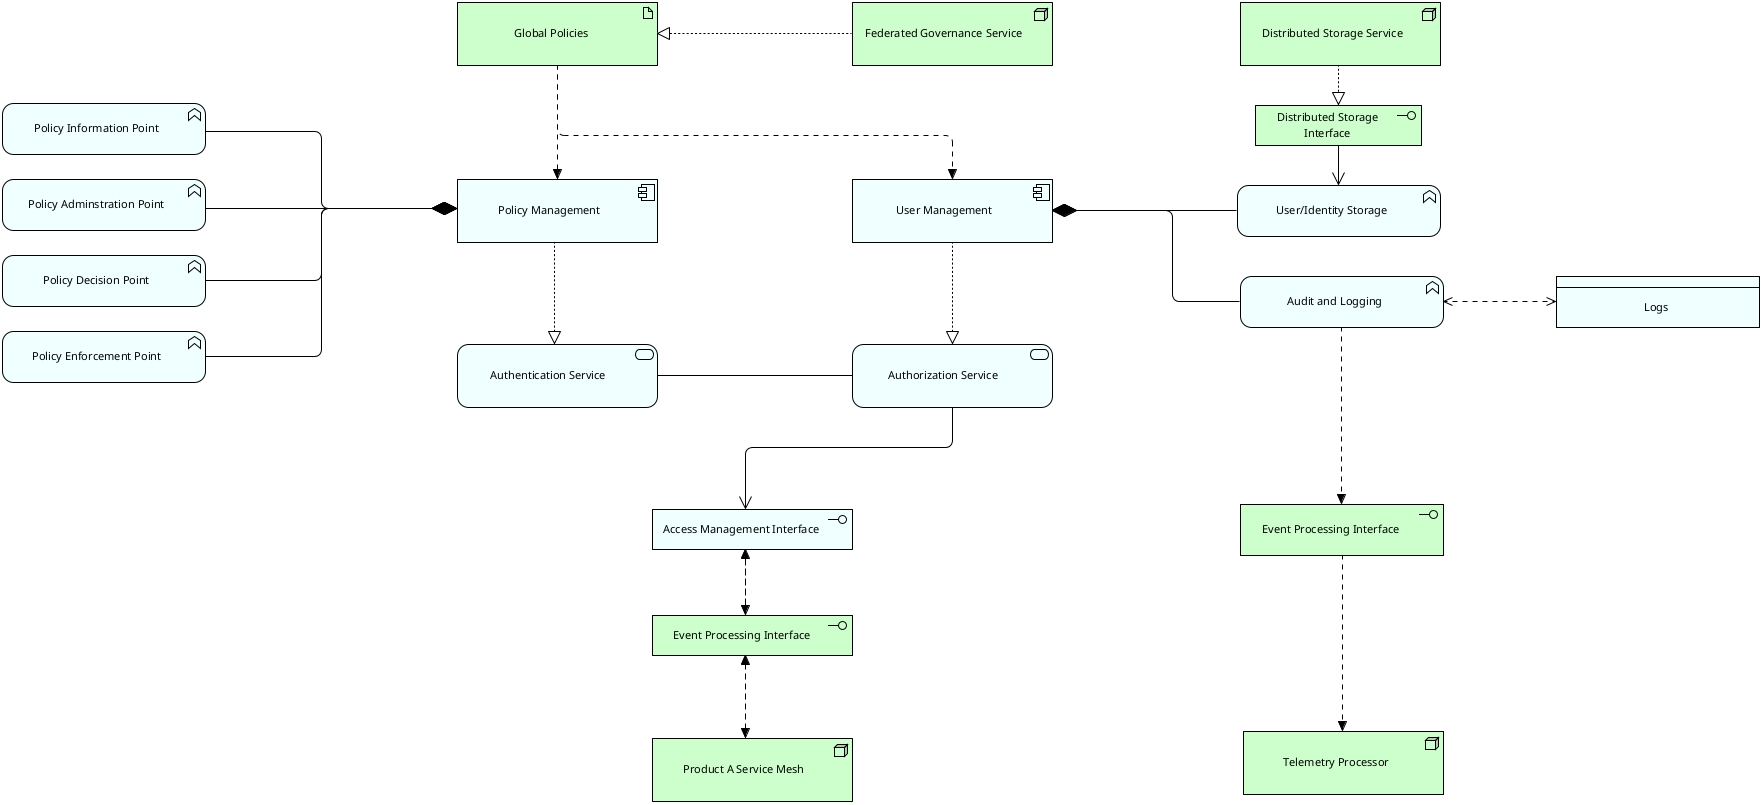
\includegraphics[width=\textwidth]{images/Metamycelium-identity-and-access-control.jpg}
        \caption{Identity and Access Control Management System}
        \label{diagram:IAM}
    \end{figure}

    \textit{Addresses requirements: SaP-1, and SaP-2.} 
    

    \item \textbf{Secret Management System:} The central secret management system is a crucial component for securely storing and maintaining sensitive information including passwords, API keys, cryptographic keys, and other secrets.
    
    The central secret management system places a strong emphasis on securely storing and encrypting secrets as a fundamental design principle. The system uses strong encryption algorithms and processes to safeguard sensitive data while it is kept, guaranteeing that confidential information is securely protected and cannot be accessed by unauthorised parties. This value aids in preventing unauthorised access to secrets, reducing the risk of data breaches, and guaranteeing confidentiality.
    
    The secret management system also facilitates the secure distribution and retrieval of secrets to authorised components or services. It offers safe APIs or client libraries that allow secrets to be retrieved securely during runtime. This value ensures that confidential information is only available to authorised entities who need it, preventing unauthorised disclosure of secrets.
    
    The secret management system also encourages integration with other components and services in Metamycelium. The system offers APIs and integration points that enable smooth integration of secrets into different data domains. This integration value enables authorised components to securely and conveniently access secrets, ensuring operational efficiency and minimising obstacles in development and deployment procedures.
    
    \textit{Addresses requirements: SaP-1, and SaP-2.} 

\end{enumerate}

The variable components in Metamycelium can be altered, adapted, or excluded according to the architect's discretion and the specific characteristics of the situation. This RA aims to enhance data architects' decision-making process by introducing established patterns and best practices from several perspectives, rather than restricting their innovation. Alternative choices for each variable module are not detailed due to the dynamic nature of the industry, and architects strive to create systems that tackle new issue areas. 

\section{Evaluation}
\label{sec:discussion}

The validation of treatment is crucial in its research, development, and implementation phase. Validating a treatment involves determining its possible impact on stakeholder objectives when applied to the specific problem at hand. 

Clearly outlining and justifying the treatment needs establishes a straightforward avenue for validation. This implies that the treatment may be verified by showing that it fulfils certain predetermined criteria. A key challenge in treatment validation is the absence of real-world implementation to assess the treatment's impact on stakeholder objectives. This challenge emphasises the need for thorough, diverse, and well-thought-out assessment methods, as discussed more in the next sections of this chapter. 

The initial phase of assessing this thesis is a single-case mechanism experiment based on the parameters outlined by \citeauthor{wieringa2014design}. Although his works reference a single experiment, this study considers a few situations. A multi-case experiment is required because the artefact is complex, which improves the thoroughness and significance of the evaluation process, leading to a more detailed and nuanced comprehension of the artifact's capabilities and possibilities. 

The research design for this case mechanism experiment is described in Section~\ref{caseMechanismResearchDesignAndValidation}. This part includes the current prototyping of the artefact and the following presentation of outcomes.


\section{Prototyping an Architecture}


Prototyping is the creation of a working model that physically represents the structure, demonstrating the design principles and ideas. This is frequently referred to as the "concrete architecture." This technique enables researchers to validate and develop the design to assess its practicality, performance, and alignment with research objectives.

Implementing the essential components and functionalities stated in the RA, Metamycelium, is part of prototyping the architecture. The selected technologies, supported by academic justification and in line with the research goals, serve as the basis for developing the prototype. The architecture's ability to manage large-scale data processing and meet various needs can be evaluated by systematically implementing its architectural components. 

Figure~\ref{metamyceliumPrototype} shows a concrete structure created with Metamycelium.

\begin{figure}[h!]
    \centering
    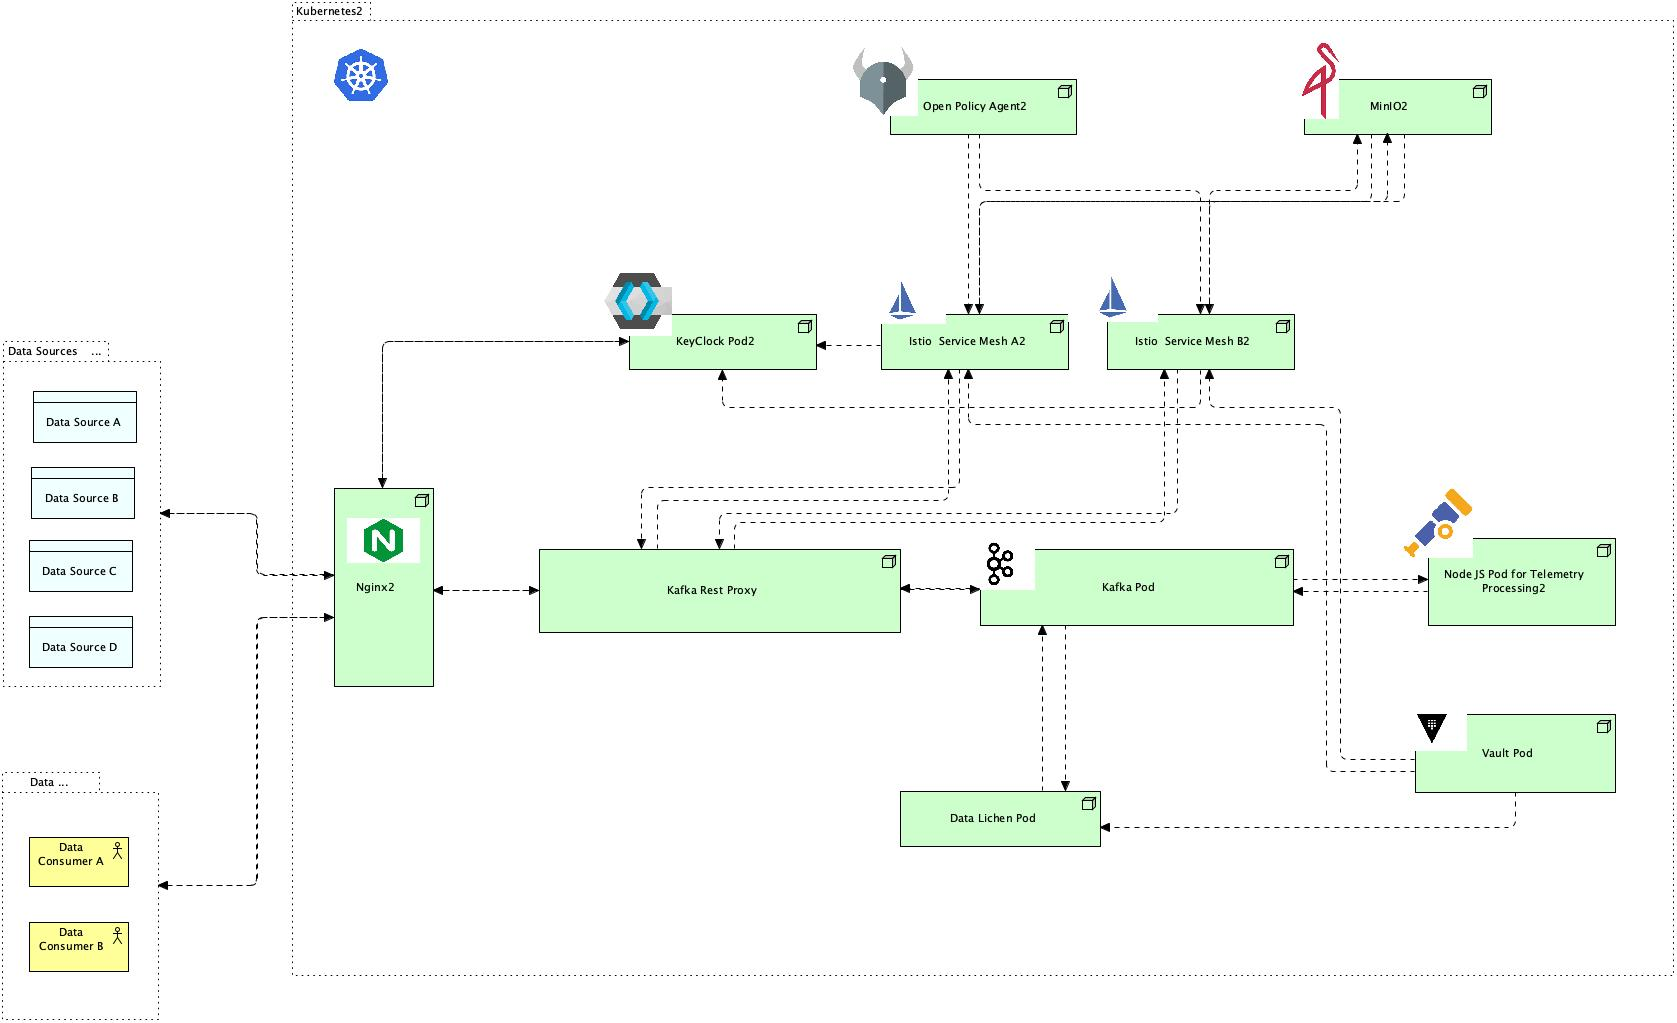
\includegraphics[width=12cm]{images/metamyceliumConcrete.jpg}
    \caption{Metamycelium Prototype}
    \label{metamyceliumPrototype}
\end{figure}

\subsection{Stage 1: Formation}


All components of this prototype are integrated within a single Kubernetes cluster. Therefore, KIND \cite{KIND2023} has been selected as the local Kubernetes cluster for this prototype to function. 


The reproducibility of this technique is crucial. The scripts required to execute, download, and set up artefacts are located in the scripts folder of the Github repository cited as \citeauthor{InfrastructureForMetamycelium2023}. These scripts are designed to exclusively operate on Unix-like operating systems.

After establishing the fundamental scripts for initialising the cluster, the procedure commenced with the creation of various services within the Kubernetes cluster. Helm Charts from Artefact Hub \cite{ArtifactHub2023} are utilised for enhanced maintainability and scalability of Nginx ingress and Kafka. Terraform was subsequently utilised to implement the charts on the Kubernetes cluster. It is located in the IaaC section of the repository. 

We conducted an extensive search for helm charts for all artefact components and selected a mature and well respected chart from Bitnami. Using this method is favoured over developing unique directives for Nginx ingress in Kubernetes and linking services to each other through Kubernetes architectural elements such as Services or StatefulSets.

The quest for charts for other components of the concrete architecture continues on Artefact Hub after the invasion. After selecting an appropriate chart for Nginx ingress, Keycloak, and Vault, the telemetry processor is established. 

Initially, a FastAPI app is set up in this procedure. The programme is containerised using Docker, hosted on Github sites, and integrated into Terraform helm release resources for deployment on the local KIND cluster. The Kubernetes ingress controller is configured as Nginx and deployed to a local type cluster using Terraform. 

Once the control setup is established, the ingress resources are configured to direct traffic to Kafka-rest-proxy. The Kafka-rest-proxy is included in the artefact to simplify the data access from the cluster. Kafka utilises a binary protocol instead of HTTP, whereas most current agents depend on HTTP for network connection. 


Once the Nginx ingress and Kafka REST proxy are properly setup, Keycloak is installed and incorporated into various components of the architecture. The Vault is integrated into the cluster using HashiCorp's official helm chart \cite{HashiCorpVaultHelm2023}. The Vault UI is active, however it is facing the obstacles outlined in Section~\ref{experimentChallenges}. 

Next, the major system to be implemented is Data Lichen. Data Lichen required a new frontend to be developed from the beginning, therefore embedded Javascript, a template engine for Node.js, was selected. This template engine was selected for its ability to simplify development and speed up the operations of this trial. 

The goal is to create a simple user interface for Data Lichen that successfully showcases the framework's potential design and capability, rather than building a comprehensive frontend. Various teams may opt to adopt Data Lichen in diverse manners. Data Lichen must be developed from the beginning because there is no existing open-source technology that offers the necessary features.

Once Data Lichen has been organised and implemented in the cluster, an Istio service mesh is established. To achieve this goal, various Kubernetes namespaces are established, and various services are categorised within the same namespace for the service mesh to manage and function. Istio's Kiali dashboard is implemented to enhance development experience and observability. 

Minio's chart is installed and the dashboard is active. The last component that needed to be deployed was Open Policy Agent (OPA). There are multiple methods to incorporate OPA into an architecture. This can be accomplished via a solo Envoy proxy, a Kubernetes operator, a load balancer with Gloo Edge, or through Istio. 

Istio was chosen because it has already been selected and deployed on the cluster. Automatically injecting policies into services inside a particular service mesh is a complex operation. The experiment involved extending the Envoy sidecar with an external authorizer API to implement inbound and outbound policies. 

Proficiency in Envoy, Kubernetes, Istio, Rego (OPA's policy language), and GoLang is essential. OPA is incorporated into the service mesh as an independent service known as a sidecar proxy. The OPA functions as an admission controller, evaluating requests sent to the Kubernetes API server. 

OPA assesses these petitions based on established policy guidelines. Approved requests are executed by the API server, whereas refused requests result in an error message sent to the user. OPA's policies manage all interactions among services and pods within a namespace. OPA assists in ensuring adherence to predetermined security and operational regulations within a Kubernetes setting. This is depicted in Figure~\ref{OPAISTIO}.

\begin{figure}[h!]
  \centering
  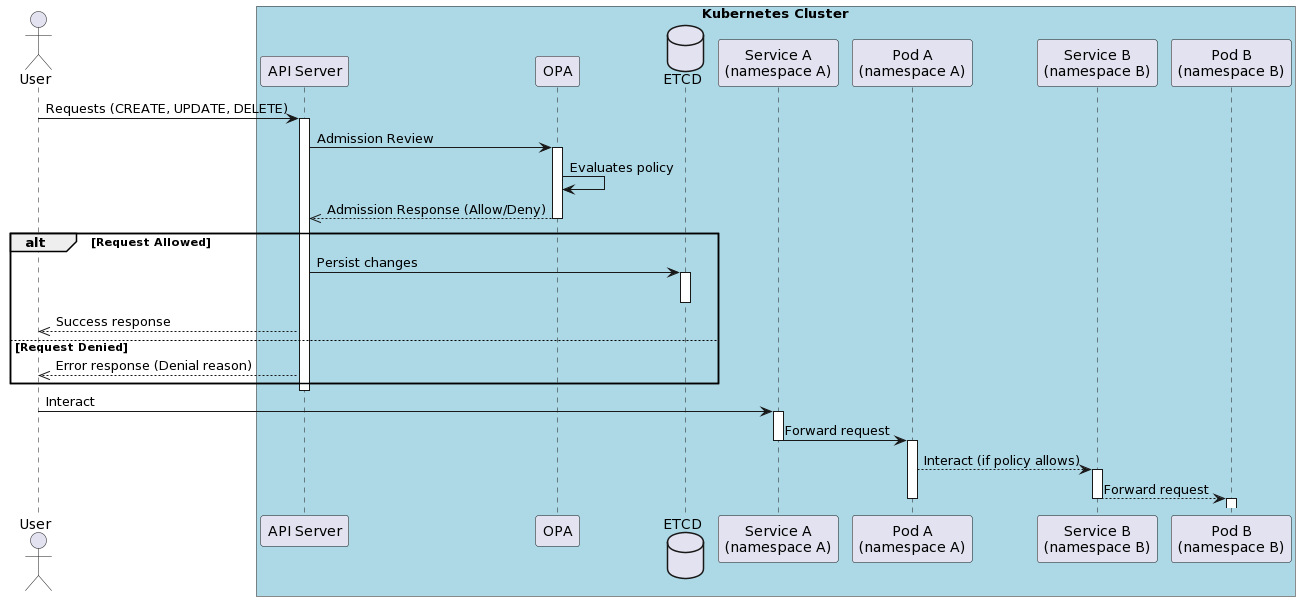
\includegraphics[width=\textwidth]{images/OPA-istio-flow.png}
  \caption{Open Policy Agent Communication Flow with Other Services}
  \label{OPAISTIO}
\end{figure}

Once OPA was understood, Domain developed an analytics service using the Python framework FastAPI. To experiment with Metamycelium and meet the requirements outlined in Section~\ref{metMyceliumRequirements}, a domain incorporating operational and analytical systems must be established. Since this experiment is not a genuine business, it is logical to establish a simulated operational service that mimics real-world activity, such as generating large amounts of data at a high speed. 

Two important data sources studied and selected for creating these domains are the Yelp Academic Dataset and the data from the U.S. Climate Resilience Toolkit's Climate Explorer. The decision is based on the extensive and detailed data provided by each source, their accessibility, and their ability to generate valuable analytical insights when utilised together.

The Yelp Academic Dataset is selected for its comprehensive compilation of restaurant reviews, containing structured and semi-structured data that encompasses customer feedback, business information, and temporal patterns. Another option, the MovieLens dataset, was found less suitable because it focuses only on movie ratings, limiting the scope of potential analysis.

The climatic Explorer dataset, which provides a detailed record of past and predicted climatic factors in the United States, is selected as an appropriate option for studying possible connections between weather trends and restaurant evaluations. Although options like Visual Crossing Weather Data Services are being examined, Climate Explorer's extensive global coverage and historical data are preferred.

The datasets qualify as big data because of their amount, variety, and velocity. The Yelp Academic Dataset comprises millions of reviews for over a hundred thousand businesses, making it a data source with a large volume and variety. The Climate Explorer dataset, updated frequently, adds a speed component to the data structure. Collectively, they offer a chance for sophisticated analytical investigations in a data-rich setting.

\subsection{Stage 2: Amalgamation}

The initial phase of developing the prototype involves establishing the foundational services within the cluster. This step focuses on establishing connections and ensuring that the architecture can effectively react to external inputs. Selected situations are applied to the system to achieve this. 

Scenarios are commonly used to evaluate new architectural designs because they offer a robust way to simulate real-world situations, allowing for the assessment of the architecture's performance in different scenarios. 

This experiment is crucial as it simulates various behaviours, system loads, data quantities, and processing kinds to analyse the architecture's resilience, adaptability, scalability, and interoperability. 

Based on the templates in Carroll (1995) and the examples in Kazman ATAM, a set of scenarios is established to evaluate the prototype's abilities. The scenarios, which include various aspects of system performance and security, are outlined in Tables \ref{s1Table} through \ref{s6Table}.

\begin{table}[tbp]
  \caption{Scenario S1: High Volume Data Ingestion Scenario}
  \begin{tabularx}{\textwidth}{|>{\raggedright\arraybackslash}p{5cm}|X|}
  \hline
  \textbf{Scenario Description:} & The system is subjected to a high volume of data, simulating peak data ingestion rates. The scenario is implemented when Domain A retrieves high volumes of data from Domain B, and processes it.  \\
  \hline
  \textbf{Relevant Quality Attributes:} & Performance, Scalability. \\
  \hline
  \textbf{Expected Outcome:} & The system can ingest, store, and process large quantities of data without significant performance degradation. \\
  \hline
  \textbf{Actual Outcome, Evaluation, Implications:} & To be filled out during testing. \\
  \hline
  \end{tabularx}
  \label{s1Table}
\end{table}

\begin{table}[tbp]
  \caption{Scenario S2: High Velocity Data Ingestion Scenario}
  \begin{tabularx}{\textwidth}{|>{\raggedright\arraybackslash}p{5cm}|X|}
  \hline
  \textbf{Scenario Description:} & The system is subjected to a high velocity of data, simulating peak data ingestion rates. The scenario is implemented when Domain A streams data into domain B and domain B stream processes the data.    \\
  \hline
  \textbf{Relevant Quality Attributes:} & Performance, Scalability. \\
  \hline
  \textbf{Expected Outcome:} & The system can ingest, store, and process continuous stream of data without significant performance degradation. \\
  \hline
  \textbf{Actual Outcome, Evaluation, Implications:} & To be filled out during testing. \\
  \hline
  \end{tabularx}
\end{table}

\begin{table}[tbp]
  \caption{Scenario S3: Data Variety Scenario}
  \begin{tabularx}{\textwidth}{|>{\raggedright\arraybackslash}p{5cm}|X|}
  \hline
  \textbf{Scenario Description:} & The system is exposed to a diverse range of data types and formats. This scenario is implemented when domain B retrieves files in different format from domain A and processes it. \\
  \hline
  \textbf{Relevant Quality Attributes:} & Variety, Interoperability. \\
  \hline
  \textbf{Expected Outcome:} & The system can handle and process different data types and formats efficiently. \\
  \hline
  \textbf{Actual Outcome, Evaluation, Implications:} & To be filled out during testing. \\
  \hline
  \end{tabularx}
\end{table}

\begin{table}[tbp]
  \caption{Scenario S4: Complex Query Scenario}
  \begin{tabularx}{\textwidth}{|>{\raggedright\arraybackslash}p{5cm}|X|}
  \hline
  \textbf{Scenario Description:} & The system processes complex queries that involve multiple large datasets. This scenario happens when an external data scientist queries both domains and tries to understand a relationship between the datasets. \\
  \hline
  \textbf{Relevant Quality Attributes:} & Computational Efficiency, Performance. \\
  \hline
  \textbf{Expected Outcome:} & The system can efficiently handle and process complex queries. \\
  \hline
  \textbf{Actual Outcome, Evaluation, Implications:} & To be filled out during testing. \\
  \hline
  \end{tabularx}
\end{table}

\begin{table}[tbp]
  \caption{Scenario S5: Secret Management Scenario}
  \begin{tabularx}{\textwidth}{|>{\raggedright\arraybackslash}p{5cm}|X|}
  \hline
  \textbf{Scenario Description:} & This scenario underscores the system's ability to manage secrets securely and efficiently, focusing on storage, retrieval, and rotation using Hashicorp Vault in conjunction with OpenID Connect's standard flow with bearer tokens. \\
  \hline
  \textbf{Relevant Quality Attributes:} & Confidentiality, Integrity, Availability. \\
  \hline
  \textbf{Expected Outcome:} & The system securely manages secrets, ensuring timely storage, retrieval, and rotation while maintaining confidentiality and integrity. \\
  \hline
  \textbf{Actual Outcome, Evaluation, Implications:} & To be filled out during testing. \\
  \hline
  \end{tabularx}
\end{table}

\begin{table}[tbp]
  \caption{Scenario S6: Data Security Scenario}
  \begin{tabularx}{\textwidth}{|>{\raggedright\arraybackslash}p{5cm}|X|}
  \hline
  \textbf{Scenario Description:} & The system's capability is evaluated regarding ensuring data security throughout access, processing, and transmission. OpenID Connect with bearer tokens is leveraged for authentication. \\
  \hline
  \textbf{Relevant Quality Attributes:} & Confidentiality, Data Integrity, Authentication. \\
  \hline
  \textbf{Expected Outcome:} & The system guarantees data security, with secure data access, processing, and transmission. Unauthorised access attempts are effectively detected and mitigated. \\
  \hline
  \textbf{Actual Outcome, Evaluation, Implications:} & To be filled out during testing. \\
  \hline
  \end{tabularx}
  \label{s6Table}
\end{table}


\subsection{Stage 3: Scenario Testing}

During this step, after defining scenarios, the system is initialised and each scenario is executed. Each specific situation is evaluated to determine how the system handles different conditions. This method entails initialising the system and methodically testing each scenario against it. 

By doing this, important measurements are recorded, leading to a more thorough comprehension of how the system reacts to different stimuli. This method assesses the system's ability to withstand challenges and its efficiency, providing valuable information about its functioning and opportunities for improvement.

\subsubsection{Scenario S1: High Volume Data Ingestion Scenario}

Before establishing the inter-domain link, it is important to review the intra-domain flow. Each operational service in the domain handles data by initially receiving an event from the analytical service and then requesting the data. The data is kept in Minio after being processed. A message is sent to a particular topic to indicate that the data storage process has been completed. 

The message is transmitted to a Kafka-rest-proxy and then to the Kafka cluster. This event contains the object's address in MinIO and other pertinent metadata. The analytics service establishes a consumer group and subscribes to a particular topic. The analytical service retrieves any new event transmitted to that topic on a background thread. 

Upon receiving the event, the analytical service utilises the metadata within the event's body to extract the object's address. Once the address is known, the analytical service directly accesses MinIO to retrieve the data. The service processes the data and saves it in an embedded SQlite database. 

The required data quality metadata from Section~\ref{section:dataQuality} and bitemporality metadata from Section~\ref{bitemporality} are generated. The metadata, service name, service address, and unique identifier are sent as an event to Kafka on a specified topic. Data Lichen establishes a consumer group, subscribes to a particular topic, retrieves the data, and subsequently presents the information for each domain. Data Lichen presents this information in a specially designed table as shown in Figure~\ref{dataLichenDashboard}. Utilising a distinct identification for each service guarantees that the listing and presentation of services are uniform and dependable, yielding consistent outcomes with every action. The flow is depicted in Figure~\ref{intraDomain}.

\begin{figure}[h!]
  \centering
  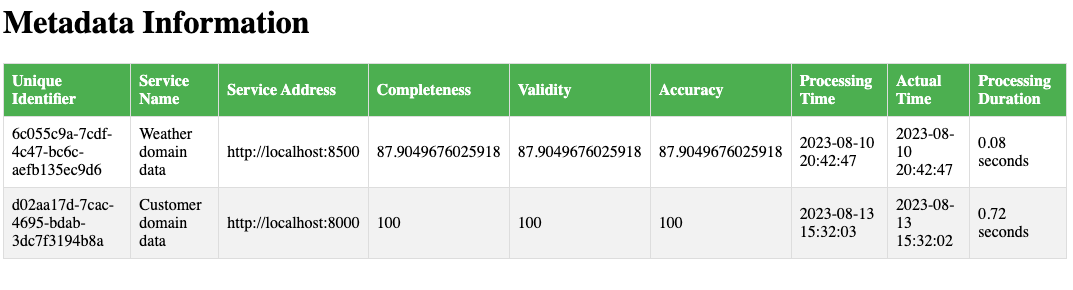
\includegraphics[width=13cm]{images/Datalichen-dashboard.png}
  \caption{Data Lichen Dashboard in Local Development Environment} 
  \label{dataLichenDashboard}
\end{figure}

\begin{figure}[h!]
  \centering
  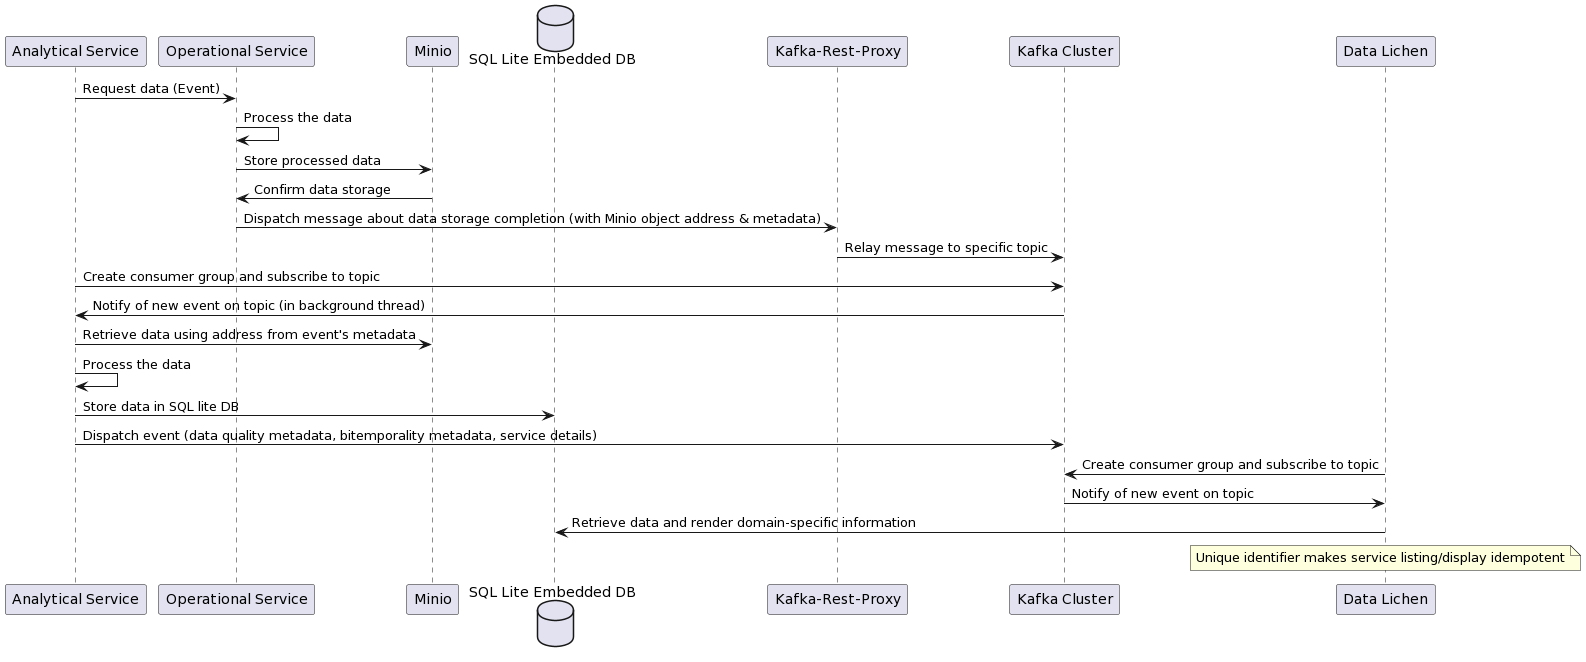
\includegraphics[width=\textwidth]{images/intra-domain-flow.jpg}
  \caption{Intra-domain communication in Metamycelium's prototype}
  \label{intraDomain}
\end{figure}

Domain A requests a 5GB JSON file from domain B in this instance. Domain A possesses the meteorological data, but domain B possesses the customer ratings and business data. An event is sent from the domain to Data Lichen to obtain a list of all datasets along with metadata such as actual-time, processing-time, completeness, and correctness. 

The information contains the address of the data domain to be retrieved. The address is utilised to send an event to domain B for data retrieval. This activates the internal process of domain B, leading to the production and storage of datasets in the distributed storage service. After the procedure is finished, an event is sent to the data processing completion topic, to which domain A is subscribed. Figure~\ref{kafkaTopics} provides an overview of the Kafka topics utilised in this investigation.

\begin{figure}[h!]
  \centering
  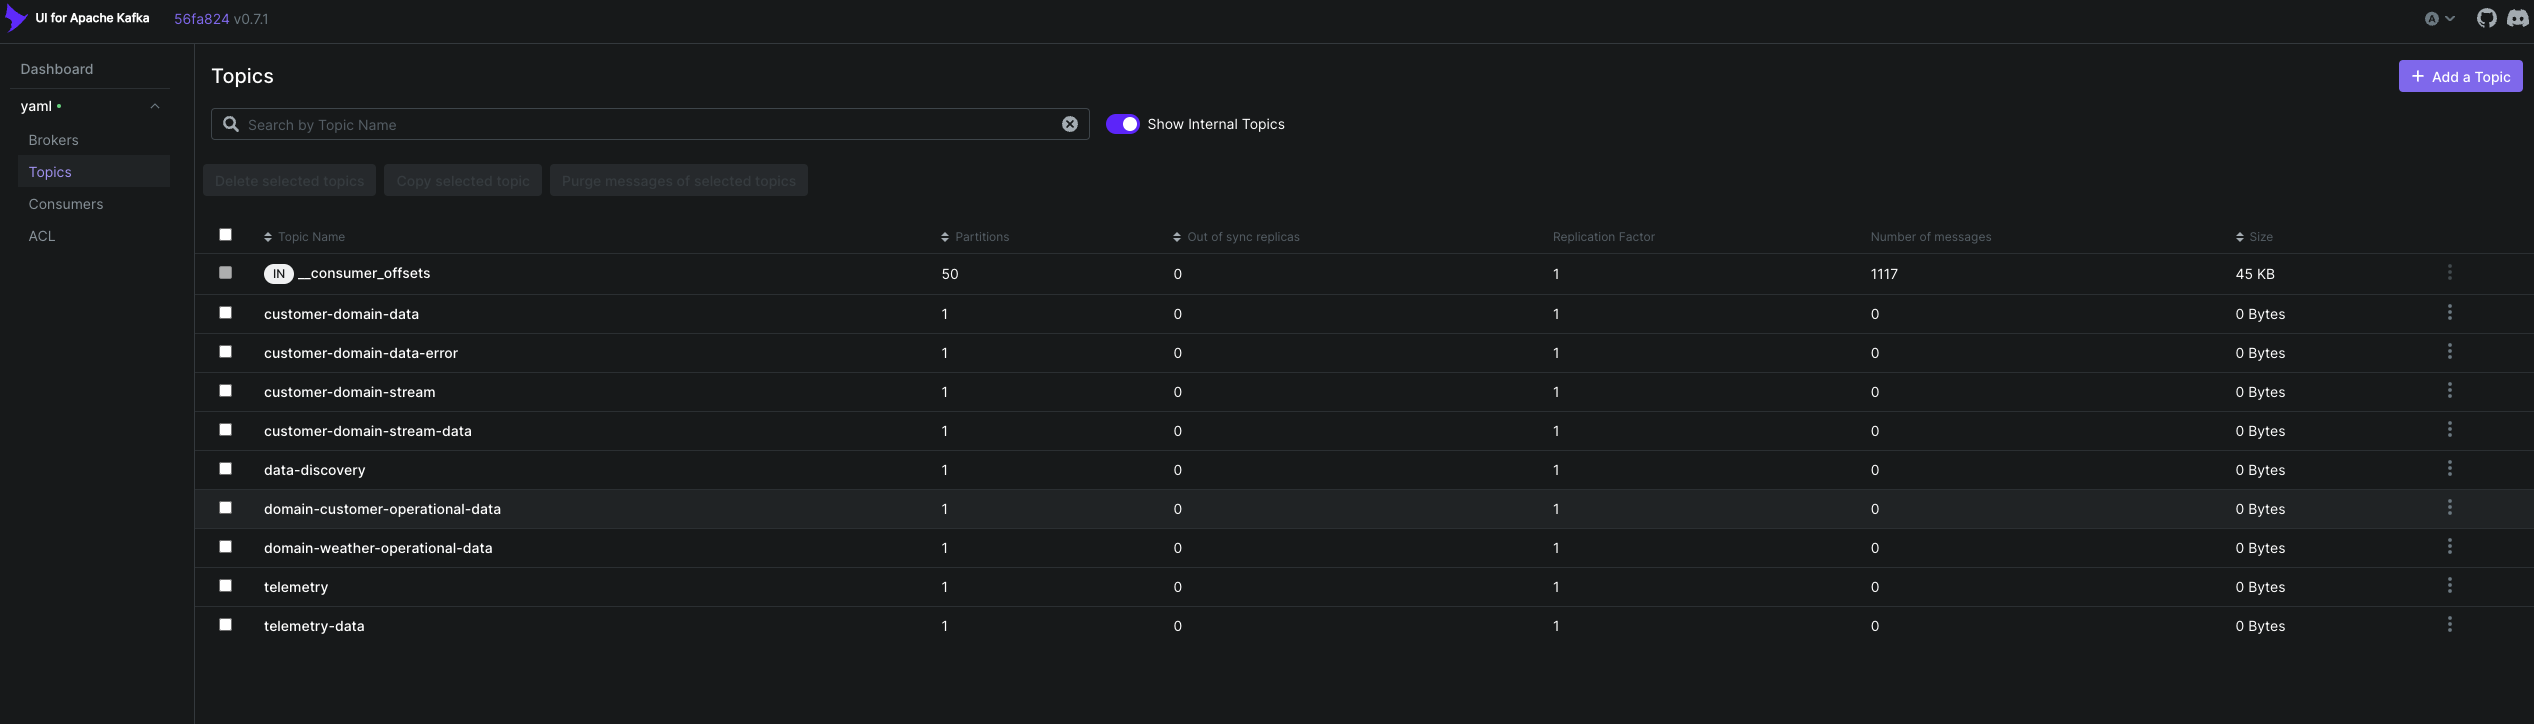
\includegraphics[width=\textwidth]{images/kafka-topics.png}
  \caption{Overview of kafka topics}
  \label{kafkaTopics}
\end{figure}

The event signalling the conclusion of data processing also includes the data address. Domain A utilises this URL to retrieve the data. After retrieving the data, it is subsequently processed. The flow is illustrated in Figure~\ref{s1Flow}.

\begin{figure}[h!]
  \centering
  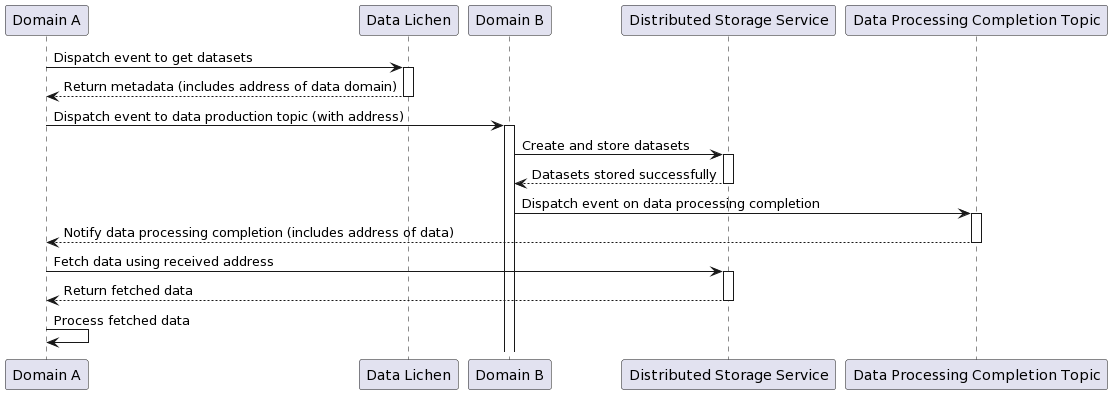
\includegraphics[width=\textwidth]{images/Scenario-s1.png}
  \caption{Scenario S-1 Flow Diagram}
  \label{s1Flow}
\end{figure}


Understanding system performance and resource utilisation is crucial in this scenario. Data Ingestion Rate is a direct indicator of the system's throughput, showing how effectively the system can handle large volumes of incoming data. A high rate indicates efficient data processing capability, crucial for situations with anticipated fast data influx. Latency, divided into intake and processing components, provides understanding of system responsiveness. Minimal latency is essential for ensuring prompt data availability and processing, especially in systems where delays can cause subsequent effects. 

CPU usage and memory utilisation are key metrics for assessing the system's resource efficiency. Increased CPU or memory usage could signal bottlenecks, inefficiencies, or places that could be optimised, particularly during times of high demand. The error rate provides information on the system's resilience and dependability. A low error rate, even with large amounts of data, indicates the system's ability to continuously manage and process data without any issues. 

These metrics collectively evaluate the system's capacity to sustain performance and stability when faced with high data input requirements. Each measure will be described in connection to the corresponding system mechanism in the following sections.

\paragraph{Data Ingestion Rate:}
Each service is instrumented using OpenTelemetry SDKs to capture telemetry data for FastAPI requests and manual spans for specified processes. The collected data is then exported to Kafka using the KafkaRESTProxyExporter class to measure the data intake rate. 

Figure~\ref{openTelemetryTopic} illustrates the open telemetry Kafka topic and a large number of events recorded in this subject. The open telemetry processor service consumes all events sent to this topic. The service gathers and maintains metrics, which are then extracted by Prometheus and subsequently sent to Grafana. The flow is depicted in Figure~\ref{openTelemetryFlow}.


\begin{figure}[h!]
  \centering
  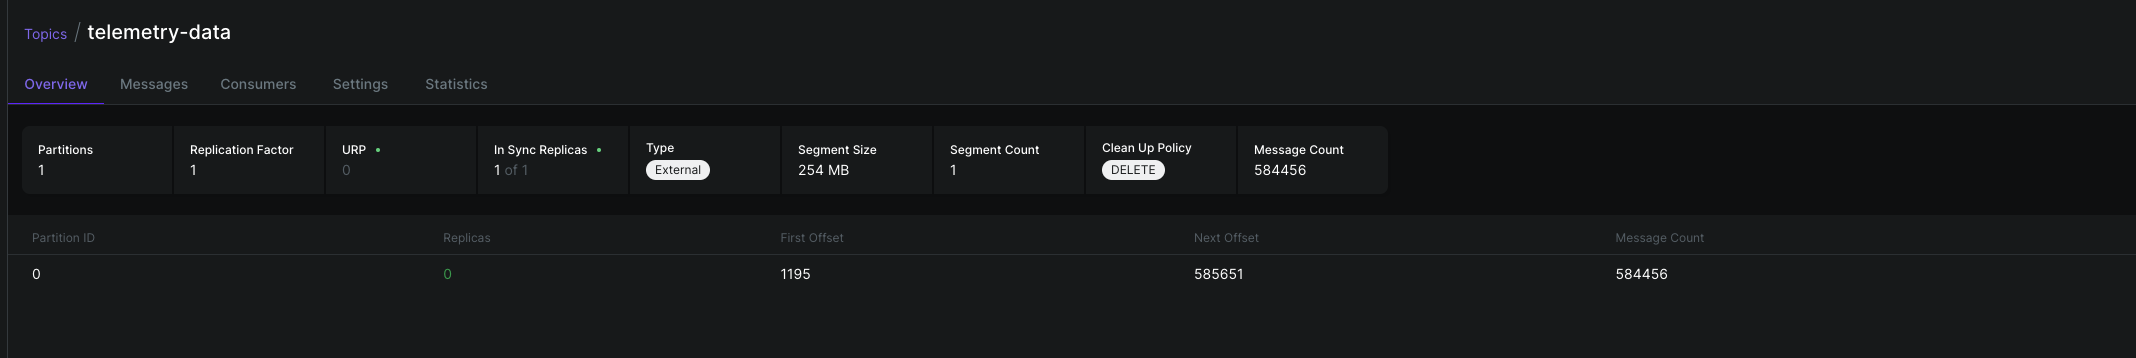
\includegraphics[width=\textwidth]{images/kafka-open-telemetry-topic-screenshot.png}
  \caption{Open Telemetry Topic}
  \label{openTelemetryTopic}
\end{figure}

\begin{figure}[h!]
  \centering
  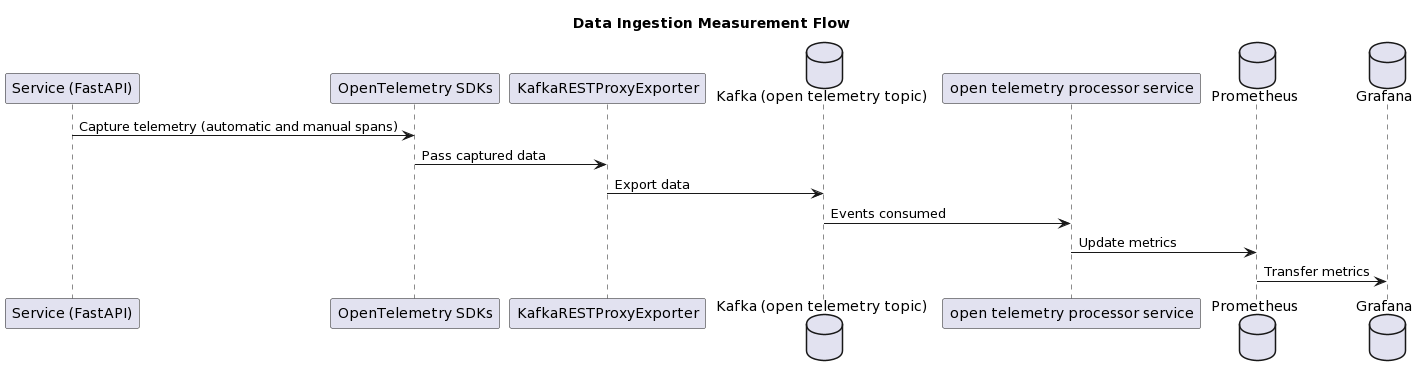
\includegraphics[width=\textwidth]{images/open-telemetry-flow.png}
  \caption{Open Telemetry Flow}
  \label{openTelemetryFlow}
\end{figure}

The JSON displayed in Figure~\ref{openTelemetryTraceSpan} depicts an example of a trace span JSON that is communicated over Kafka to the open telemetry service.

\begin{figure}[h!]
  \centering
  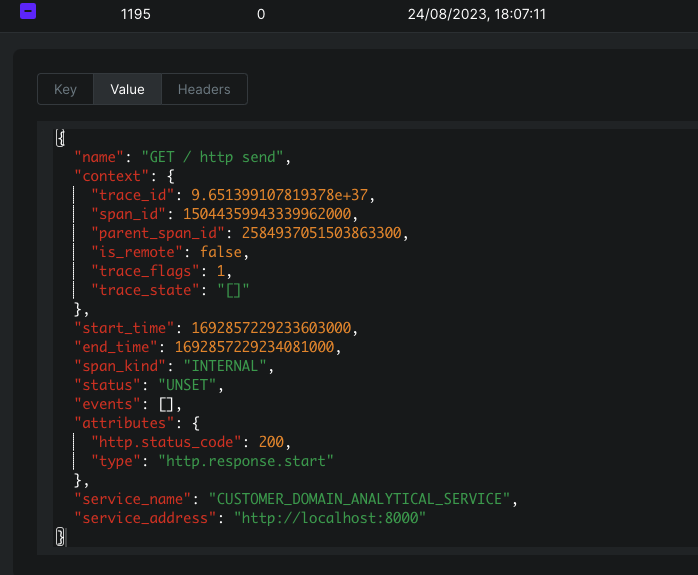
\includegraphics[width=\textwidth]{images/open-telemetry-trace-example.png}
  \caption{Open Telemetry Trace Span}
  \label{openTelemetryTraceSpan}
\end{figure}

Before presenting the experiment results, it is crucial to define the specific meaning of 'heavy load of data' in the context of this study. In BD, there is no commonly accepted criterion for defining "high volume," particularly in decentralised, domain-driven architectures such as Metamycelium. There is no single standard benchmark that universally defines what qualifies as a heavy data load in these systems. 

Academic research and business reports suggest that daily data intake can reach terabytes or more, particularly in high-velocity streams such as social media or e-commerce transactions. 

Transferring many gigabytes of data in JSON format between domains is a substantial stress test due to its verbosity and demands compared to binary formats. The Yelp academic dataset is divided into 400KB chunks and transferred many times to test the prototype's capability and resilience against increased data traffic. 

This configuration is suitable for practical scenarios where systems need to consistently handle continuous streams of incoming data from different sources and varying quantities, while maintaining high performance and data integrity. Metamycelium's decentralised, event-driven architecture is designed to allow data to be smoothly ingested, processed, and retrieved, regardless of the frequency of dataset transfers or accesses. This assesses the system's capacity to manage large amounts of data and its ability to perform well in a setting that replicates the rapid data flow typical of modern big data scenarios.


All data sent during the experiment is stored in MinIO. Upon successful storage, a confirmation is always sent back. The process of streaming, storing, and validating data was repeated several times to demonstrate its reliability, especially when dealing with large amounts of data. Reliable and accurate communication in challenging situations supports the importance of consistent communication in remote systems, as shown in academic research such as Kleppmann (2017). The process can be formally represented using logical implications to determine the system's resilience.

Let's denote the following:
\begin{itemize}
    \item \( P \) as the event where ``data is transferred from Domain A to Domain B''.
    \item \( Q \) as the event where ``data is successfully stored in MinIO''.
    \item \( R \) as the event where ``confirmation of successful storage is communicated back''.
\end{itemize}

From the empirical observations, it is deduced that:
\[ P \implies Q \]
\[ Q \implies R \]

Thus, utilizing the transitive property of implications \cite{johnson2019logic}, it is inferred that:
\[ P \implies R \]




\section{Discussion}
\label{sec:discussion}
% Reflect on the findings from the evaluation, discussing their implications, limitations, and the relevance to existing and future research.

\section{Conclusion}
\label{sec:conclusion}
% Summarize the main contributions of your paper, its practical implications, and suggest directions for future research.




\appendix




\bibliographystyle{elsarticle-harv}
\bibliography{bibfile}

\end{document}
\endinput
%%
%% End of file `elsarticle-template-num.tex'.